
\documentclass[twocolumn,linenumbers]{aastex631}

\newcommand{\vdag}{(v)^\dagger}
\newcommand\aastex{AAS\TeX}
\newcommand\latex{La\TeX}


\usepackage{gensymb}
\usepackage{amsmath}
\usepackage{array}
\usepackage{tabularx}
\usepackage{xfrac}
\definecolor{limegreen}{HTML}{32CD32}

\newcommand{\fidsim}{\mathtt{SNeRHD}}

\begin{document}
\author{Thummim Mekuria}
\affiliation{Department of Astronomy and Astrophysics \\
University of California, Santa Cruz CA,95064, USA} \textcolor{magenta}{(needs input: add a second, CCA affiliation here too?)}

\author{Shyam Menon}
\affiliation{\textcolor{magenta}{needs full affiliation (currently just "rutgers")}}
\affiliation{\textcolor{magenta}{needs full affiliation (currently just "cca")}}

\author{Michael Y. Grudi\'{c}}
\affiliation{\textcolor{magenta}{needs full affiliation (currently just "cca")}}

\author{Nia Imara}
\affiliation{Department of Astronomy and Astrophysics \\
University of California, Santa Cruz CA,95064, USA}

\author{Piyush \textcolor{magenta}{(needs full name)}}
\affiliation{\textcolor{magenta}{needs real affiliation -- currently just "ask"}}

\author{rachel \textcolor{magenta}{(needs full name)}}
\affiliation{\textcolor{magenta}{needs full affiliation (currently just "cca")}}

\title{Outflows from a starburst galaxy at Cosmic Dawn}
\begin{abstract}
The overabundance of UV-bright galaxies at Cosmic Dawn---``blue monsters'' --- challenges galaxy evolution models calibrated on the low-redshift universe. Analytical models have proposed efficient bursts of star formation along the removal of gas and dust by stellar feedback, as potential mechanisms for producing these galaxies. We present three-dimensional radiation hydrodynamic simulations of a dense gas cloud embedded in a $10^{11} M_\odot$ halo that investigate the competition between star formation and feedback in realistic high-redshift conditions. All simulation runs reach star formation efficiencies of $\sim 65\%$ within two freefall times (5 Myr). The systems reach a peak SFR of $ > 50\ M_\odot\ \mathrm{yr^{-1}}$ at $t\sim 3$ Myr. Once the stars begin to go supernova at $t\sim 6$ Myr, $2.5\times 10^9\ M_\odot$ of gas and dust are dispersed in radiatively-inefficient outflows. \textcolor{magenta}{decide: report the higher-metallicity runs here as both 0.1 and 1 $Z_\odot$, or just solar for direct comparison to the MW?} At the fiducial metallicity of $0.01 Z_\odot$, $30 \%$ of the outflowing gas is in the hot ionized phase, with velocities of $\geq 3v_\mathrm{esc}$. The remaining two-thirds of the gas is in the warm neutral and warm ionized phases, which have velocities of $\sim 0.5v_\mathrm{esc}$. Because the winds clear dust along with the gas, $\gtrsim 80\%$ of the UV photons escape the system unattenuated, leaving behind a system with a rest-frame $M_\mathrm{UV} \approx -25\ \mathrm{mag}$. Therefore a physically-motivated set of initial conditions and feedback prescriptions can produce a UV-bright starburst having properties consistent with those observed at Cosmic Dawn.
\end{abstract}

\section{Introduction}
The James Webb Space Telescope (JWST) has enabled the spectroscopic confirmation and characterization of galaxies out to redshifts $z > 11$, providing unprecedented observational access to galaxy formation during the first billion years of the universe (e.g., \citealt{2023Natur.622..707A, 2023A&A...677A..88B, 2025A&A...697A..90B, 2026arXiv260111515D,2025arXiv251212813H}). The JWST-constrained UV luminosity function (UVLF) exceeds predictions by semi-analytic models and hydrodynamic simulations calibrated on the local universe \citep{2025arXiv251012411M, 2026arXiv260202322M,2025arXiv250804791F,2024MNRAS.531..997C, 2026MNRAS.546f2267C, 2025ApJ...995...43A, 2025A&A...698A.234D,2024ApJ...960...56H, 2025arXiv250804791F,2020ApJ...891..146R,2024A&A...691A..87M,2026arXiv260121833H}; this discrepancy persists even after recalibration across independent modelling frameworks, both semi-analytic and hydrodynamic, which continue to under-predict the abundance of UV-bright galaxies at $z\gtrsim10$ \citep{2025A&A...696A.157M,LagosShark2026}.
% there is an overabundance of massive ($M \geq 10^9 M_\odot$), UV-bright ($M_{\mathrm UV} \lesssim -22.5\ \mathrm{mag}$), and blue ($-2.0 < \beta_\mathrm{UV} < -2.9$) galaxies at $z =8–10$ 

The appearance of such UV-bright galaxies by 500 Myr after the Big Bang does not by itself imply that they are massive, since stellar and halo masses remain difficult to pin down. Their brightness could instead arise from efficient mass assembly (a high star formation efficiency), a dust-free environment, which yields more observed light for a given stellar mass, or a top-heavy IMF or AGN contribution, which produce more UV light for a given stellar mass. Their colors further suggest unobscured young stellar systems. Highly efficient star formation, a top-heavy IMF, and a dust-free environment have been proposed as likely explanations for the abundance of these systems \citep{2022ApJ...938L..10I,2023MNRAS.522.3986F,2023MNRAS.523.3201D,2023ApJ...955L..35S,2024A&A...684A.207F,2023MNRAS.520.2445Z,Somerville2025SFE}. \cite{2023MNRAS.523.3201D} argue that the enhanced density $n>3\times10^3\ \mathrm{cm^{-3}}$ and low metallicity $Z<0.1 Z_\odot$ of the early universe lead to gas free-fall times of $t \sim 1$ Myr, which are much shorter than the time for feedback processes---such as jets, winds and supernovae--- to turn on. This leads to a star formation efficiency of $\epsilon \sim 1$, such that a $10^{11}\ M_\odot$ halo at $z=10$ would host a galaxy with $M_*\sim 10^{10}\ M_\odot$.
% sfr of 65 msun/yr, stellar mass of 1e11 msun

\citet{2023MNRAS.522.3986F} propose that once high-$z$ galaxies cross a critical specific star formation rate threshold of $25 \ \mathrm{Gyr}^{-1}$, feedback-driven winds expel the interstellar gas and dust from these galaxies, significantly reducing the attenuation and reddening of UV photons from the young stellar population \citep{2023MNRAS.520.2445Z,2024A&A...684A.207F}. The extremely blue slopes and near-unity Lyman continuum escape fractions measured in individual systems lend observational support to this scenario \citep{2026arXiv260202322M, 2025OJAp....8E.125F, 2024ApJ...976..160H, 2025A&A...698A.234D,2023ApJ...955L..35S}. 

The initial gas surface density is critical for setting the freefall time of the gas and determining the force balance between gravity and stellar feedback. Cloud-scale simulations of star cluster formation show that gravitational collapse is unimpeded by feedback for gas past a critical surface density threshold of $\Sigma \geq 10^3 M_\odot \mathrm{pc^{-2}}$ \citep{2023MNRAS.521.5160M,2025ApJ...987...12M,2019MNRAS.483.5548G}. \cite{2023MNRAS.521.5160M} show that star formation efficiencies of $\geq 70-80\%$ can be reached for an initial gas cloud of $M =10^6\ M_\odot$. These results are consistent with analytical predictions \citep{2010ApJ...710L.142F,2018MNRAS.473.3717F,2019MNRAS.488.1501G}.

\cite{2023MNRAS.521.5160M} also show that once high SFEs are reached, the impulse from UV radiation reprocessed by dust becomes super-Eddington and launches outflows with $v_\mathrm{out} \sim 0.5-2 v_\mathrm{esc}$. However, there is a separation of 3 orders of magnitude in mass that prevents direct bridging of the results of cloud-scale simulations to analytical models explaining blue monsters (e.g., \citealt{2023MNRAS.523.3201D,2023MNRAS.522.3986F}). 
Additional galactic physics, such as the dark matter potential and thermodynamic interactions with the interstellar medium, must also be considered. 

In this work, we present three-dimensional radiation hydrodynamic simulations of a dense cloud embedded in a $10^{11} M_\odot$ halo at $z=10$, in order to investigate the balance between feedback and gravity at galaxy-scales. We model the evolution of an isolated gas cloud with $M = 1.7\times 10^{10}\ M_\odot$, radius of $R=700\ \mathrm{pc}$ and fiducial metallicity $Z=10^{-2}Z_\odot$ over a period of 20 Myr ($8t_\mathrm{ff}$). We run a suite of simulations parameterized by the feedback physics included and the metallicity of the gas.

The paper is organized as follows: in Section 2 we describe the equations solved and code used, as well as the initial conditions, and the suite of simulations to test parameter space. In Section 3, we begin with an overview of the general evolution of the gas, then provide detailed analysis of the phase structure of the ISM as a function of feedback physics and metallicity. We also calculate the escape fraction of UV photons from the simulated system. In Section 4, we compare our results to the literature, both observations and theory, then make predictions for how the simulated galaxies might evolve to lower-redshift counterparts. We also discuss caveats and numerical convergence tests in this section, then end with a summary in Section 5.


\section{Methods}
\subsection{Equations solved}
We solve the equations of non-relativistic radiation hydrodynamics coupled to non-equilibrium chemistry. The radiation treatment follows \citet{2023MNRAS.521.5160M}, to which we refer the reader for details, with three differences. First, the isothermal equation of state of that work is replaced by an explicit gas energy equation, with net heating and cooling computed from the chemical network. Second, we evolve three ultraviolet bands rather than a single UV band and a dust-reprocessed IR band. Third, the sink particles inject supernova feedback in addition to radiation.

The gas obeys
\begin{align}
& \frac{\partial \rho}{\partial t} + \nabla \cdot (\rho \mathbf{v}) = \dot{\rho}_\mathrm{SNe} - \dot{\rho}_\mathrm{acc} \label{eq:mass}\\
& \frac{\partial (\rho \mathbf{v})}{\partial t} + \nabla \cdot (\rho \mathbf{vv}) = -\nabla P - \rho \nabla \Phi + \sum_\lambda \mathbf{G}_\lambda \label{eq:momentum}\\
& \frac{\partial E_\mathrm{g}}{\partial t} + \nabla \cdot \left[(E_\mathrm{g} + P)\mathbf{v}\right] = -\rho \mathbf{v} \cdot \nabla \Phi + \mathbf{v} \cdot \sum_\lambda \mathbf{G}_\lambda \nonumber\\
& \qquad\qquad + \rho(\Gamma - \Lambda) + \dot{E}_\mathrm{SNe} \label{eq:energy}\\
& \frac{\partial (\rho X_i)}{\partial t} + \nabla \cdot (\rho X_i \mathbf{v}) = \rho \dot{X}_i \label{eq:species}\\
& \nabla^2 \Phi = 4\pi G (\rho + \rho_*), \label{eq:poisson}
\end{align}
where $\rho$ is the gas mass density, $\mathbf{v}$ the gas velocity, $P$ the thermal pressure, $\Phi$ the gravitational potential, and $\rho_*$ the mass density of the sink particles. $\dot{\rho}_\mathrm{acc}$ is the removal of gas by accretion onto sink particles, and $\dot{\rho}_\mathrm{SNe}$ and $\dot{E}_\mathrm{SNe}$ are the supernova mass and energy source terms defined below. The total gas energy density is $E_\mathrm{g} = \rho e + \rho v^2/2$, where $e$ is the specific internal energy. Equation \ref{eq:energy} is equivalent to evolving $\rho e$ under advection, $P\,\mathrm{d}V$ work, viscous (shock) heating at discontinuities and the source terms on its right-hand side. $\Gamma$ and $\Lambda$ are the specific heating and cooling rates. The radiation force on the gas in each band is $\mathbf{G}_\lambda$ (Equation \ref{eq:G}). \textcolor{limegreen}{(needs to be double-checked) (1) the code evolves total energy as written here, given \texttt{eintSwitch} = $10^{99}$ in flash.par, whose comment says to set it to zero; (2) energy absorbed by dust leaves the gas and only $\mathbf{v}\cdot\mathbf{G}_\lambda$ is added (\texttt{rt\_hydro\_type} = 1, radiative equilibrium); (3) the supernova energy is injected thermally, not kinetically. If kinetic, Equation \ref{eq:momentum} also needs a supernova term.}

The mass fractions $X_i$ of 18 species (e$^-$, H, H$^+$, H$_2$, H$_2^+$, H$_3^+$, He, He$^+$, He$^{2+}$, C, C$^+$, CH, O, O$^+$, OH, CO, CO$_\mathrm{ice}$ and HCO$^+$) are advected with the gas and evolved by a non-equilibrium reaction network solved with KROME \citep{2014MNRAS.439.2386G} \textcolor{limegreen}{(needs to be double-checked) the species list looks like the Gong+17 network}, which also returns $\Gamma$ and $\Lambda$. The network includes the local radiation field in each band, along with a constant background radiation field and cosmic-ray ionization rate. \textcolor{limegreen}{(needs to be double-checked) the list of heating and cooling processes. The run inputs include H$_2$, CO, OH, H$_2$O and collisional-ionization-equilibrium metal cooling tables.}

The system is closed with a multi-species ideal-gas equation of state,
\begin{align}
P = (\gamma_\mathrm{eff} - 1)\rho e = \frac{\rho k_\mathrm{B} T}{\mu m_\mathrm{H}},
\end{align}
where the mean particle weight $\mu$ and the effective adiabatic index $\gamma_\mathrm{eff}$ follow from the local composition,
\begin{align}
\frac{1}{\mu} = \sum_i \frac{X_i}{A_i}, \qquad \frac{1}{\gamma_\mathrm{eff} - 1} = \mu \sum_i \frac{X_i}{A_i (\gamma_i - 1)}.
\end{align}
Here $A_i$ is the atomic mass of species $i$, with $\gamma_i = 5/3$ for atomic and ionic species and $\gamma_i = 1.4$ for molecular species. The sound speed is then $c_s^2 = \gamma_\mathrm{eff} P / \rho$, so that unlike in an isothermal treatment, it varies with the local thermal and chemical state of the gas.

The radiation field is evolved in three bands, $\lambda \in$ (EUV, LW, PE), corresponding to the extreme ultraviolet ($h\nu > 13.6$ eV), Lyman-Werner ($11.2 < h\nu < 13.6$ eV) and photoelectric ($6 < h\nu < 11.2$ eV) ranges. We use the mixed-frame moment equations of \citet{2023MNRAS.521.5160M} and \citet{2022MNRAS.512..401M}, retaining terms of leading order in all limiting regimes of radiation hydrodynamics:
\begin{align}
& \frac{\partial E_{r,\lambda}}{\partial t} + \nabla \cdot \mathbf{F}_\lambda = j_{*,\lambda} - cG^0_{v,\lambda} \\
& \frac{\partial \mathbf{F}_\lambda}{\partial t} + \nabla \cdot (c^2 \mathbf{P}_{r,\lambda}) = -c^2 \mathbf{G}_\lambda,
\end{align}
where
\begin{align}
G_{v,\lambda}^0 = \ & \rho \kappa_{\mathrm{P},\lambda} E_{r,\lambda} + \rho (\kappa_{\mathrm{R},\lambda} - 2\kappa_{\mathrm{P},\lambda}) \frac{\mathbf{v} \cdot \mathbf{F}_\lambda}{c^2} \nonumber\\
& + \rho (\kappa_{\mathrm{P},\lambda} - \kappa_{\mathrm{R},\lambda}) \left[ \frac{v^2}{c^2} E_{r,\lambda} + \frac{\mathbf{vv}}{c^2} : \mathbf{P}_{r,\lambda} \right]
\end{align}
and
\begin{align}\label{eq:G}
\mathbf{G}_\lambda = \rho \kappa_{\mathrm{R},\lambda} \frac{\mathbf{F}_\lambda}{c} - \rho \kappa_{\mathrm{R},\lambda} E_{r,\lambda} \frac{\mathbf{v}}{c} - \rho \kappa_{\mathrm{R},\lambda} \frac{\mathbf{v}}{c} \cdot \mathbf{P}_{r,\lambda}.
\end{align}
Here $E_{r,\lambda}$, $\mathbf{F}_\lambda$ and $\mathbf{P}_{r,\lambda}$ are the lab-frame radiation energy density, flux and pressure tensor, $\kappa_{\mathrm{P},\lambda}$ and $\kappa_{\mathrm{R},\lambda}$ are the Planck and Rosseland mean opacities, and $j_{*,\lambda}$ is the emission from the sink particles. Since dust does not re-emit at these energies, there is no diffuse emission term in any of the three bands, and photons absorbed in a band are removed from the radiation field. Unlike \citet{2023MNRAS.521.5160M}, we do not evolve an infrared band, so radiation pressure from dust-reprocessed infrared photons is not included (see Section \ref{sec:ir_caveat}). The dust opacities are fixed in each band, at $\kappa_\mathrm{d} = 1250$, $900$ and $514\ \mathrm{cm^2\ g^{-1}}$ for EUV, LW and PE respectively, and scale linearly with metallicity. The EUV band also includes absorption by H and H$_2$, with cross-sections $\sigma_\mathrm{H} = 3.1\times10^{-18}\ \mathrm{cm^2}$ and $\sigma_\mathrm{H_2} = 4.6\times10^{-18}\ \mathrm{cm^2}$.

We close the moment equations with a variable Eddington tensor,
\begin{align}
\mathbf{P}_{r,\lambda} = \mathbf{T}_\lambda E_{r,\lambda},
\end{align}
where $\mathbf{T}_\lambda$ is computed from angular quadratures of the specific intensity $I_{r,\lambda}(\mathbf{\hat{n}}_k)$,
\begin{align}
&E_{r,\lambda} = \int d\Omega\, I_{r,\lambda}(\mathbf{\hat{n}}_k) / c \\
&\mathbf{P}_{r,\lambda} = \int d\Omega\, \mathbf{\hat{n}}_k \mathbf{\hat{n}}_k I_{r,\lambda}(\mathbf{\hat{n}}_k) / c,
\end{align}
and $I_{r,\lambda}$ follows from the formal solution of the time-independent transfer equation,
\begin{align}
\frac{\partial I_{r,\lambda}}{\partial s} = \frac{j_{*,\lambda}}{4\pi} - \rho \kappa_{\mathrm{R},\lambda} I_{r,\lambda}.
\end{align}

Sink particles represent unresolved stellar populations that emit radiation and detonate supernovae according to their mass and age. Each sink emits as a Gaussian source,
\begin{align}
j_{*,\lambda}(r) = \frac{L_{*,\lambda}}{(2\pi\sigma_*^2)^{3/2}} \exp\left(-\frac{r^2}{2\sigma_*^2}\right),
\end{align}
where $r$ is the distance from the sink, $\sigma_* = 4\Delta x$, $\Delta x$ is the cell size, and $L_{*,\lambda} = \Psi_\lambda(t_\mathrm{age}) M_*$. The light-to-mass ratios $\Psi_\lambda$ evolve with the age of the population following Starburst99 \citep{1999ApJS..123....3L} \textcolor{limegreen}{(needs to be double-checked) the IMF and tabulation metallicity}. For a newly formed sink, $\Psi_\lambda \approx 500$, $110$ and $280\ L_\odot\ M_\odot^{-1}$ for EUV, LW and PE. $\Psi_\mathrm{EUV}$ remains constant for about 3 Myr and then declines, while $\Psi_\mathrm{LW}$ and $\Psi_\mathrm{PE}$ rise by a factor of about 2 over the same period before declining.

Supernovae begin at a sink age of $3.7$ Myr, at a rate $\dot{N}_\mathrm{SNe} = \dot{n}_\mathrm{SNe}(t_\mathrm{age}) M_*$, with a specific rate $\dot{n}_\mathrm{SNe} \approx (3-5)\times10^{-4}\ M_\odot^{-1}\ \mathrm{Myr^{-1}}$ over the ages reached in our simulations. Each supernova injects $10^{51}$ erg of energy within a radius of $4\Delta x$ of the sink, along with $\sim 10\ M_\odot$ of ejecta, which is removed from the sink, giving the $\dot{E}_\mathrm{SNe}$ and $\dot{\rho}_\mathrm{SNe}$ terms in Equations \ref{eq:mass} and \ref{eq:energy}.


\subsection{Numerical Tools}
we solve the above equations using $\mathtt{FLASH}$ \citep{2000ApJS..131..273F,2008PhST..132a4046D}\\
$\mathtt{VETTAM}$\cite{2022MNRAS.512..401M}

We make the following choices in solving these equations numerically:
\begin{itemize}
    \item subgrid star formation prescription: starburst99
    \item  The number of supernovae at each timestep is calculated as 
$ N_\mathrm{SNe} = \dot{n}_\mathrm{SNe} M_* \Delta t$, where $\dot{n}_\mathrm{SNe}$ is the specific supernova rate, $M_*$ is the sink-particle mass, and $\Delta t = 0.1\ \mathrm{Myr}$ is the timestep. 
    \item The number of supernovae, the radiation field, and the timing of the first supernova all depend on the IMF, stellar evolution models, and stellar multiplicity, each of which carries well-known uncertainties.
    \item When supernovae detonate, each one injects $10^{51}$ erg of thermal energy and $\sim 10\ M_\odot$ of ejecta mass into the ISM; momentum is not injected directly but builds up dynamically as the remnant sweeps up the surrounding gas.
    \end{itemize}

\subsection{Initial conditions + parameters}
\textcolor{limegreen}{(needs to be double-checked) which parameters were chosen independently (and from which literature) and which were derived; how the 700 pc radius and $M_\mathrm{g}$ were set. The section then needs to connect to the galaxies in the Introduction}
\begin{itemize}
    \item $M_\mathrm{halo} = 10^{11} M_\odot$, $z=10$. At this redshift, the baryon fraction is \textcolor{magenta}{needs input: what baryon-fraction value (and assumed $\Omega_b/\Omega_m$) was actually used here?} $f_b$, which gives an initial gas mass of $1.7\times10^{10}\ M_\odot$ (Section 1)
    \item \textcolor{limegreen}{(needs to be double-checked) "based on some factor" does not say what the factor is or where it comes from -- what is the Schechter-formalism-based factor that sets $R=700$ pc, and what initial surface density does that give? Also still needs its own observational citation -- it is not \citet{Somerville2025SFE} (arXiv:2505.05442), which is about density-modulated star formation efficiency and the UVLF, not baryon concentration radii; that paper is now cited instead in the Introduction, where it belongs} The Schechter formalism gives the virial radius, and assuming the baryons are concentrated in the central zone based on some factor gives the radius of a sphere with $R=700\ \mathrm{pc}$, which in turn gives the gas an initial surface density of \textcolor{magenta}{()}.
    \item \textcolor{magenta}{sentence fragment, missing value: "turbulent velocity fluctuations of ()"} the cloud is also initialized with turbulent velocity fluctuations of ().
    \item \textcolor{limegreen}{(needs to be double-checked) summarize the results from the IMF experiment here -- light-to-mass ratio and supernova rates depend on the IMF, and we should state our assumptions and acknowledge that conditions here are very different from the local universe where the IMF is measured}
    \end{itemize}

% \begin{table*}
%     \centering
%     \begin{tabular}{|c||c|}
%     \hline
%       Property& Value\\
%      \hline 
%      \hline
%      $M_\mathrm{*}$& $10^{11}\ M_\odot$\\
%      $M_\mathrm{halo}$& $1.7 \times 10^{10}\ M_\odot$\\
%      R& 700 pc\\
%      z& 10\\
%  Z&0.01 $Z_\odot$\\
%  \hline
%     \end{tabular}
%     \caption{\textcolor{magenta}{Caption}}
%     \label{tab:tab1}
% \end{table*}



\subsection{Simulation suite}
Table \ref{tab:tab1} summarizes the simulations analyzed in this work. The runs are differentiated based on the feedback physics and metallicity. At the fiducial metallicity ($0.01Z_\odot$), we run four physics cases--no feedback ($\mathtt{HD}$), radiation only ($\mathtt{RHD}$), supernovae only ($\mathtt{SNe}$) and both radiation and supernovae ($\mathtt{SNeRHD,f}$). We also model the full physics runs at two higher metallicities: $\mathtt{SNeRHD,0.1Z_\odot}$ and $\mathtt{SNeRHD,Z_\odot}$. The lower metallicity runs are performed at two resolutions, $N = 128$ and $N = 256$, to test convergence. 
Joint analysis of this suite of simulations enables us to isolate the individual contributions of radiation and supernova feedback to the dynamics of the gas, and examine how the metal and dust content determine its thermal evolution.\\

\begin{table*}
    \centering
    \begin{tabular}{|c||c|c||c|c|}
    \hline
 Model& \multicolumn{2}{c|}{Feedback Physics}& Metallicity&Resolution\\
    % \hline
      &  Radiation &   Supernovae & $Z_\odot$& \\
     \hline 
     \hline
     $\mathtt{HD}$ &  -&   -&$10^{-2}$& $128^3$, $256^3$\\
     $\mathtt{RHD}$ &  $\checkmark$&   -&$10^{-2}$& $128^3$, $256^3$\\
     $\mathtt{SNe}$ &  -&   $\checkmark$&$10^{-2}$& $128^3$, $256^3$\\
     $\mathtt{SNeRHD,f}$&  $\checkmark$&   $\checkmark$&$10^{-2}$& $128^3$, $256^3$\\
 $\mathtt{SNeRHD,0.1Z}_\odot$& $\checkmark$& $\checkmark$&  $10^{-1}$&$128^3$\\
 $\mathtt{SNeRHD,Z}_\odot$& $\checkmark$& $\checkmark$& 1&$128^3$\\
 \hline
    \end{tabular}
    \caption{Summary of the simulation suite. Columns give the model name, whether radiation and supernova feedback are included, the gas metallicity in units of $Z_\odot$, and the grid resolution of each run.}
    \label{tab:tab1}
\end{table*}

\section{Results}
We begin with a general overview of the fiducial run (3.1), then discuss the comparative effects of radiation and supernova feedback physics on setting the star formation efficiency (3.2). We examine the bulk kinematics (3.3) and thermodynamical phase structure (3.4) of the feedback-driven outflows. We examine how the metallicity of the gas affects the phase structure of the outflows (3.5), and photon escape fractions (3.6).

\subsection{General evolution}
% \textcolor{red}{the velocity vectors need to be less numerous / more visible - decrease the frequency and increase size for the quivers.put back the x/y ticks (1.kpc etc).for all the figures: make fontsize bigger -- make comparable to the  in overleaf}
\begin{figure}[ht!]
    \centering
    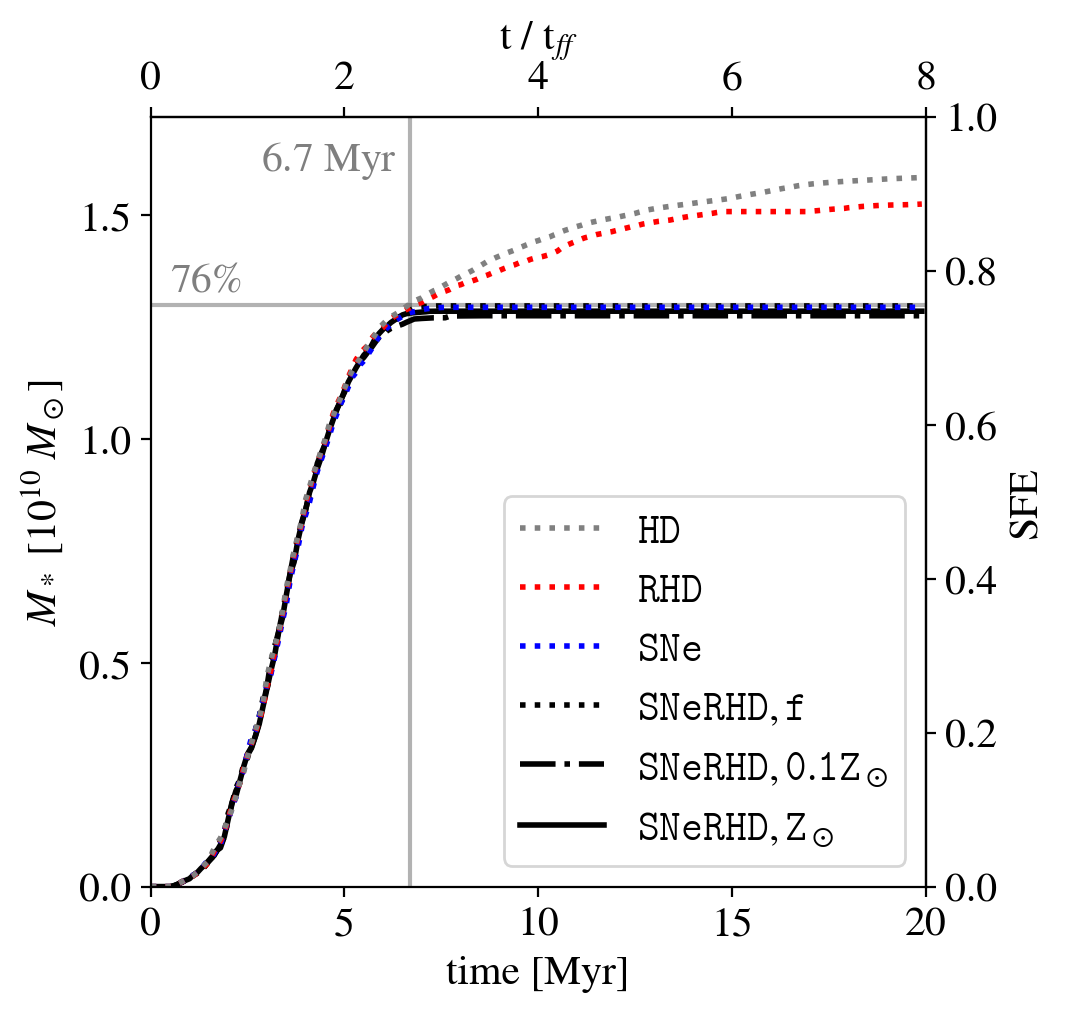
\includegraphics[width=\linewidth]{fig1_mstar.png}
    \caption{Star formation efficiency of the simulation runs presented in this work (Table 2). The color of each line indicates the feedback physics included, while the linestyle encodes the metallicity of the gas. The vertical dashed line indicates the detonation of the first supernova at t = 6.3 Myr. The horizontal dashed line shows the peak SFE achieved by the fiducial run $\mathtt{SNeRHD,f}$.}
    \label{fig:mstar_runs}
\end{figure}

\begin{figure*}[ht!]
    \centering
    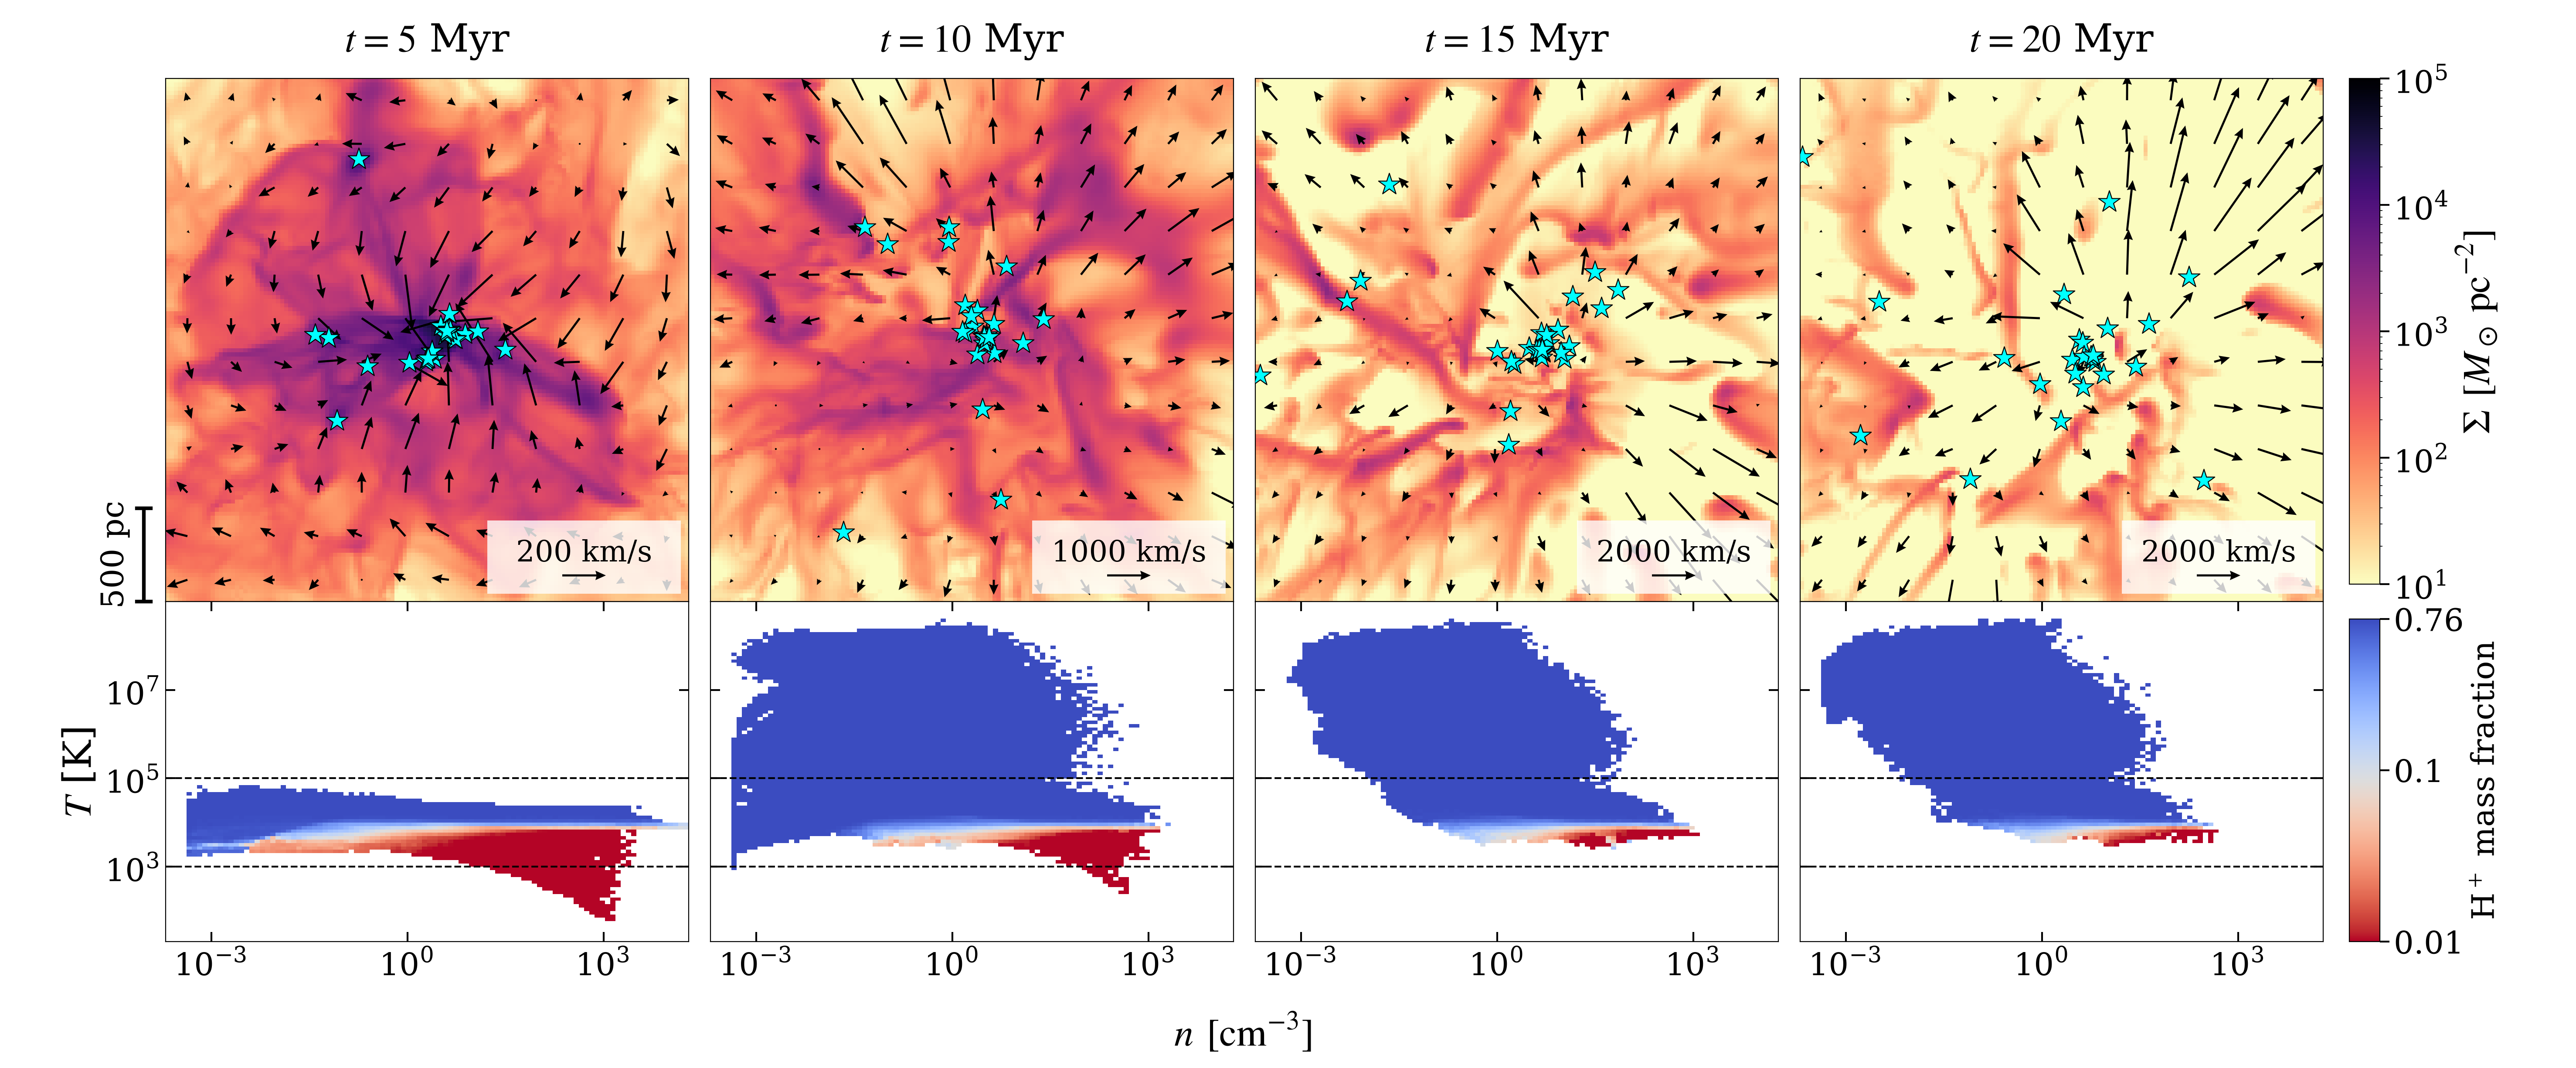
\includegraphics[width=\linewidth]{fig2_snapshots.png}
    \caption{Snapshots of the fiducial simulation at t = 5, 10, 15, and 20 Myr. Top row: projected gas surface density, with the mass-weighted gas velocity shown as arrows (the key in each panel gives that panel's scale) and star clusters marked as cyan stars. Bottom row: the phase of the ISM in density--temperature space, colored by the mass-weighted H$^+$ mass fraction. The horizontal dashed lines indicate the demarcation between the cold, warm, and hot phases.}
    \label{fig:mstar_evolution}
\end{figure*}

We show the evolution of the fiducial run in two complementary ways. Figure \ref{fig:mstar_evolution} follows the gas surface density and phase structure in snapshots, while Figure \ref{fig:mstar_runs} collapses the spatial information into the stellar mass formed, which samples the evolution densely in time.

Whether feedback can halt the collapse is set by the ratio of the outward force that feedback exerts on the gas to the inward force of gravity. Per unit stellar mass, this ratio is
\begin{align}\label{eq:Gamma}
    \Gamma = \frac{\langle \dot{p}/M_*\rangle_\mathrm{rad} + \langle \dot{p}/M_*\rangle_\mathrm{SNe} + \langle \dot{p}/M_*\rangle_\mathrm{other}}{4\pi G\Sigma},
\end{align}
where $\Sigma$ is the surface density of the gas, and the terms in the numerator are the specific momentum injection rates from radiation pressure, from supernovae, and from mechanisms not modelled here, such as radiation pressure from dust-reprocessed infrared photons, Lyman-$\alpha$ resonant scattering and protostellar jets (Section \ref{sec:caveats}). Feedback can halt the collapse when $\Gamma > 1$. Before the first supernovae detonate, the only feedback in our simulations is the radiation pressure of UV photons absorbed by dust, $\langle \dot{p}/M_*\rangle_\mathrm{rad} = L_\mathrm{UV}/(M_* c)$, which gives
\begin{align}\label{eq2:Guv}
    \Gamma_\mathrm{UV} = \frac{L_\mathrm{UV}/M_* }{4\pi c G\Sigma}.
\end{align}
Cloud-scale RHD simulations \citep{2024ApJ...967L..28M} show that radiation feedback is unable to regulate star formation in gas that has surface densities exceeding $\Sigma_\mathrm{crit} \sim 10^3 M_\odot \mathrm{pc^{-2}}$, at which the outward pressure exerted on the gas by UV photons absorbed by dust is balanced by the inward pressure from gravitational collapse.
In the above expression, the specific UV luminosity of a newly formed star cluster is $L_\mathrm{UV}/M_* = 900\ L_\odot M_\odot^{-1}$ (for a Chabrier IMF). $\Sigma$ is the surface density of gas in the ISM, G is the gravitational constant, and c is the speed of light. Gas with surface densities in excess of $\Sigma_\mathrm{crit} \gtrsim 10^3 M_\odot\ \mathrm{pc^{-2}}$ would have $\Gamma_\mathrm{UV}$ less than unity, favoring gravitational contraction. 

Given the initial conditions of the cloud, the gas freefall time is $t_\mathrm{ff} \approx 2.5\ \mathrm{Myr}$, and the snapshots in Figure \ref{fig:mstar_evolution} are taken at $t = (2,4,6,8) \times t_\mathrm{ff}$, which correspond to 5, 10, 15, and 20 Myr. The evolution of the fiducial run, $\fidsim$, falls into three eras, which we describe in turn from the perspective of the stars and then of the gas.

\textit{Gravitational collapse ($t < t_\mathrm{det} = 6.3$ Myr).} The first star clusters form within the first 1 Myr. Because the gas surface density exceeds $\Sigma_\mathrm{crit}$, $\Gamma_\mathrm{UV} < 1$ and star formation proceeds essentially unimpeded: by $5\ \mathrm{Myr}$, $1.1\times10^{10}\ M_\odot$ of star clusters ($64\%$ of the initial gas mass) have already formed, primarily in the center of the domain. The gas, meanwhile, is dominated by gravitational contraction, aided by supersonic shocks that compress it into dense filaments. At 5 Myr it is undergoing global radial infall, and the filaments funnel gas into the center of the domain, fueling continued star formation.

\textit{Supernova onset ($t_\mathrm{det} < t \lesssim 10$ Myr).} Once the first supernovae detonate, star formation stops, and the stellar mass plateaus at $\epsilon_* \approx 0.76$ (Figure \ref{fig:mstar_runs}). For the gas, feedback now dominates over gravity: by 10 Myr, its large-scale velocity is radially outward.

\textit{Dispersal ($10-20$ Myr).} No new stars form, and the star clusters remain as a tightly bound system. The feedback-driven winds remove $\sim 1.5\times 10^9\ M_\odot$ of gas between 10 and 15 Myr, leaving behind diffuse tendrils in place of dense filaments. An additional $4\times 10^8\ M_\odot$ of gas is lost between $15-20$ Myr, and the remaining gas is at the periphery and moving outward. By $t= 20$ Myr, there is $2\times 10^8\ M_\odot$ ($1\%$ of $M_\mathrm{g,0}$) left in the simulation box, around an unobscured set of star clusters.

In the following section, we discuss the relative contributions of radiation and supernova feedback in shaping the dispersal of the interstellar medium (ISM).
\subsubsection{Bulk properties of outflows}\label{sec:bulk}
\begin{figure*}[ht!]
    \centering
    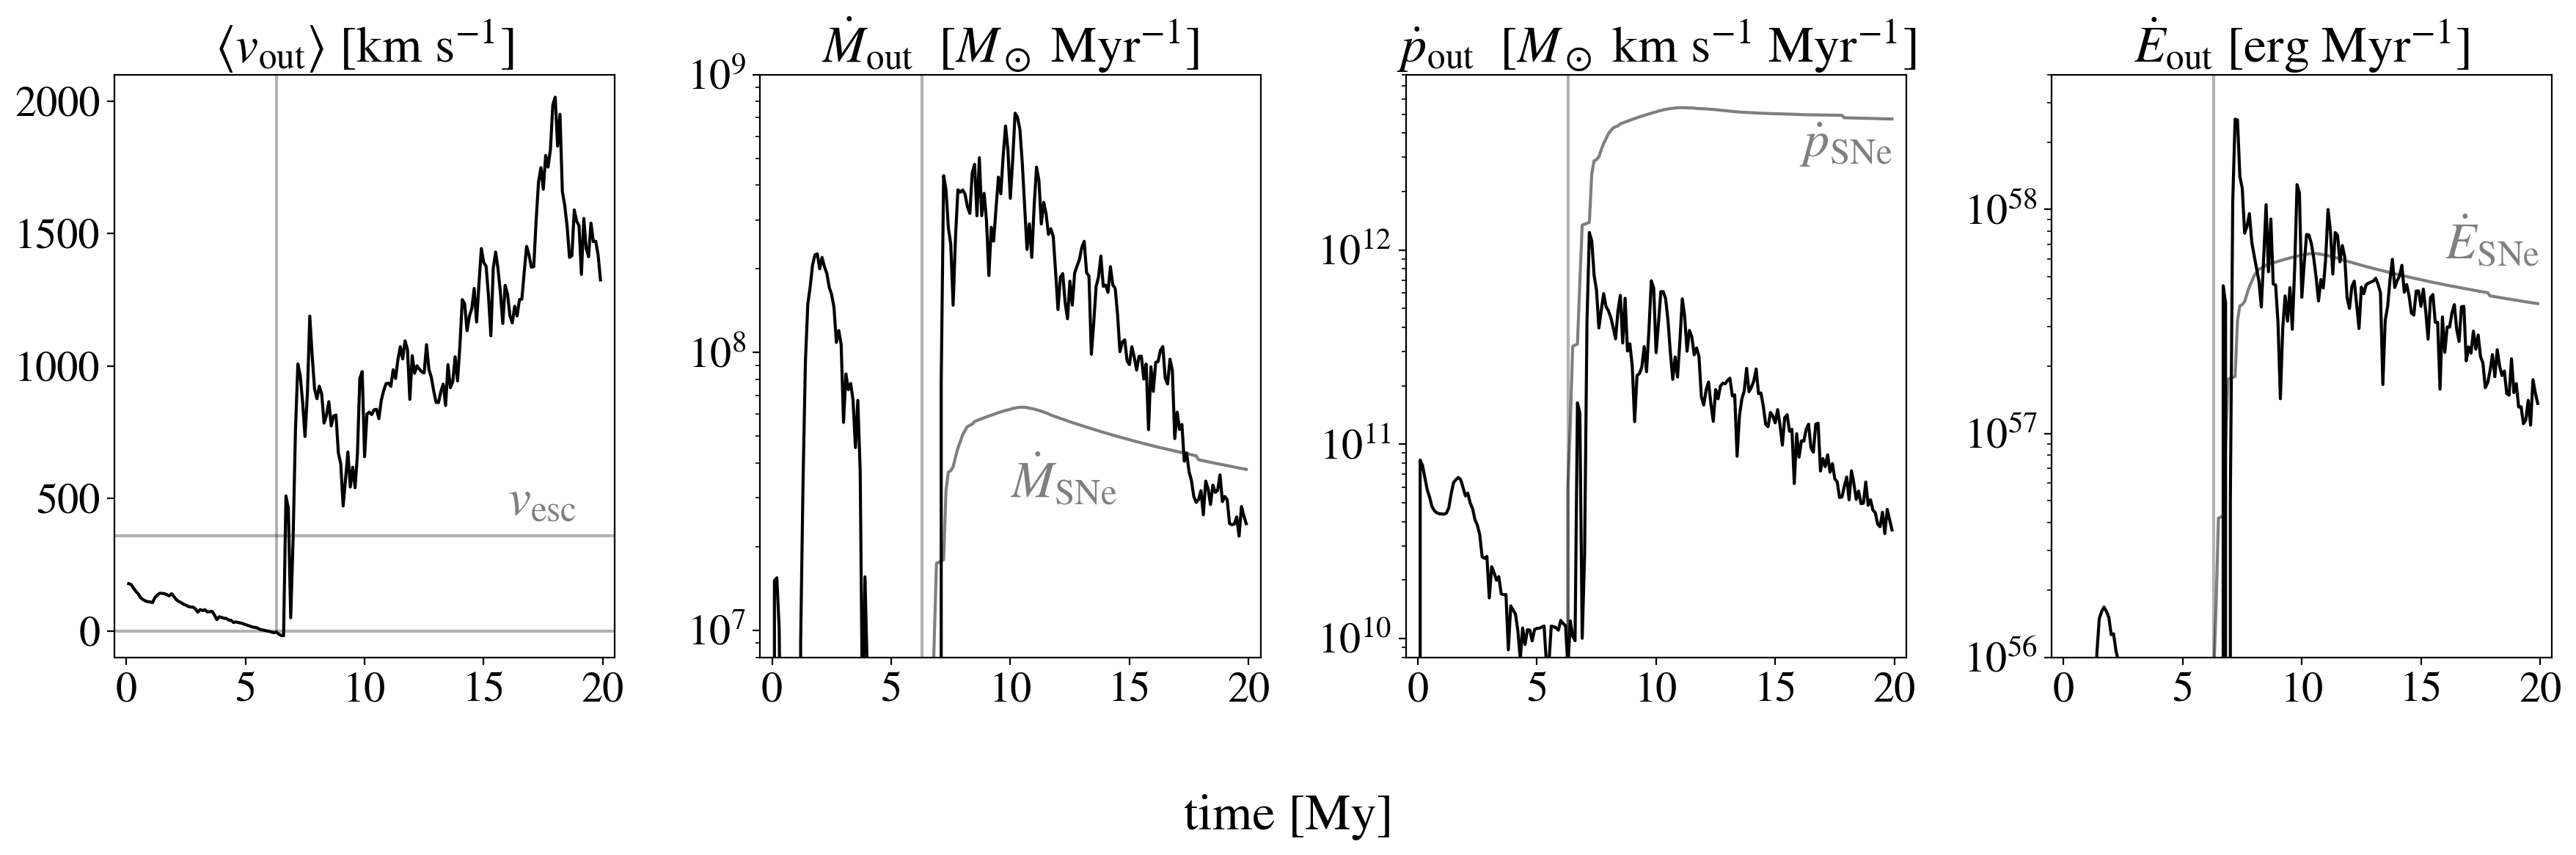
\includegraphics[width=\linewidth]{fig2.png}
    \caption{Bulk properties of the feedback-driven outflows in the fiducial simulation, with the vertical line marking $t_\mathrm{det}$. From left to right, the panels show a) the average velocity, b) mass outflow rate, c) momentum outflow rate and d) energy outflow rate.  The grey horizontal line in panel a) shows the escape velocity from the gravitational potential at r = 1kpc ($665\ \mathrm{km\ s^{-1}}$, including both the baryons and the dark matter halo). The grey lines in panels b-d are reference values calculated from the analytically derived expectations of the momentum and energy shed into the interstellar medium from detonating supernovae.
    % \textcolor{red}{rearrange this+6,7 to be m,v,p,e, add a) b) c) d)}
    }
    \label{fig:outflow_rates}
\end{figure*}

Once the first supernovae detonate at $t_\mathrm{det}$, gas is driven out of the cloud. To quantify this, we measure the flux of mass, momentum and energy through a closed surface around the starburst, beginning with the mass. The mass flux of gas through a surface in the simulation box is given by: 
\begin{align}
    \dot{M}_\mathrm{out} = \int_{\partial S} \rho \ (v \cdot \hat{n})\ dA
\end{align}
where $\rho$ is the mass density of gas in each cell, $v$ is its velocity, and $\hat{n}$ is the unit vector outward normal to the surface $\partial S$. The integral is evaluated over a spherical surface at $r = 1$ kpc, matching the surface used throughout the rest of the paper (e.g.\ Figures \ref{fig:phase_diagram} and \ref{fig:outflow_phases}), similar to \cite{2023MNRAS.521.5160M}. 

Figure \ref{fig:outflow_rates} shows the temporal evolution of $\dot{M}_\mathrm{out}$ through a surface at $r = 1\ \mathrm{kpc}$ in the fiducial run. An initial peak in $\dot{M}_\mathrm{out}$ occurs at $t \sim 2$ Myr from turbulent velocity fluctuations in the gas, which are subsequently damped as gravity begins to dominate and accretes gas back toward the center of the simulation. A second, more prominent spike of $\dot{M}_\mathrm{out}$ occurs at $t \sim 6$ Myr, shortly after the first supernovae detonate.

Due to the continuous deposition of momentum by the supernovae, a steady outflow rate of $\langle \dot{M}_\mathrm{out} \rangle \sim 3\times 10^8 M_\odot \ \mathrm{Myr^{-1}}$ is maintained for about 5 Myr. After $t = 13$ Myr, $\dot{M}_\mathrm{out}$ begins to decline, as there is progressively less gas left in the domain interior to $r = 1\ \mathrm{kpc}$ (Figure \ref{fig:mstar_evolution}). 
% \textcolor{red}{compare to \citep{2026ApJ..1000..158C}}

The mass-averaged outflow velocity is given by:
\begin{align}
\langle v \rangle _\mathrm{out} = \frac{\int_{\partial S} \rho \ (v \cdot \hat{n})\ \mathcal{H}(v\cdot \hat{n})(v\cdot \hat{r})\ dA}{\int_{\partial S} \rho \ (v \cdot \hat{n})\ \mathcal{H}(v\cdot \hat{n})\ dA},
\end{align}
where $\mathcal{H}$ denotes the Heaviside step function applied to $v \cdot \hat{n}$ to filter for gas with a net outward velocity. 

During the initial gravitational collapse phase, the gas has velocities well below the $v_\mathrm{esc}$ of the system. Once the supernovae detonate, this changes nearly instantaneously, with the gas accelerated to $\langle v \rangle _\mathrm{out} \sim 1000\ \mathrm{km\ s^{-1}}$ at $t \sim 7$ Myr. As the amount of gas left in the simulation decreases with time, the supernovae impart a larger specific momentum to the gas. By t = 20 Myr, the outflows have $\langle v \rangle _\mathrm{out} \gtrsim 1500\ \mathrm{km\ s^{-1}}$, more than twice the escape velocity of the system.

Figure \ref{fig:outflow_rates} also shows the momentum and energy rates of the outflows, which we calculate as:
\begin{align}
    \dot{p}_\mathrm{out} &= \int_{\partial S}\ \rho \ (v \cdot \hat{n}) (v \cdot \hat{r})\ dA \\
    \dot{E}_\mathrm{out} &= \int_{\partial S}\ \rho \ (v \cdot \hat{n})\ (\frac{v^2}{2} + \ \ e_\mathrm{int})\ dA.
\end{align}

Here $\hat{r}$ is the radial unit vector, $e_\mathrm{int}$ is the specific internal energy of the gas, and $dA$ is the area element of the surface. The first (second) term in the integrand of $\dot{E}_\mathrm{out}$ correspond to the kinetic (thermal) energy of the gas. Both the momentum and energy flux exhibit behavior qualitatively similar to $\dot{M}_\mathrm{out}$, rising sharply following the onset of supernovae and subsequently declining as gas is expelled from the system. 

To compare these outflow rates with the energy and momentum available from feedback, we need the rate at which supernovae detonate. The rate of supernovae, $\dot{N}_\mathrm{SNe}$, in the simulations is insensitive to radiation and metallicity, rising steeply to a peak of $6.4\times10^6\ \mathrm{Myr}^{-1}$ at $10.5\ \mathrm{Myr}$ across all the runs. After this, the rate of detonation declines as the massive stars have died off, reaching to $\dot{N}_\mathrm{SNe} \sim 4\times10^6\ \mathrm{Myr}^{-1}$ at the simulation end time of $20\ \mathrm{Myr}$. Each supernova deposits an average kinetic energy of $10^{51}\ \mathrm{erg}$ into the ISM, along with $\sim 10 M_\odot$ of stellar material as ejecta. % \textcolor{red}{this propagates through the surrounding gas and pushes on it outward}

The terminal momentum injected into the ISM by a supernova depends on the ambient density and metallicity \citep{2018MNRAS.480..800H}, who calibrate this against single-supernova-remnant simulations including those of \citet{1988ApJ...334..252C}:
\begin{align}
p_t &\approx 4.8\times 10^5 \left(\frac{E_\mathrm{ej}}{10^{51}\ \mathrm{erg}}\right)^{13/14}\left(\frac{n_b}{\mathrm{cm^{-3}}}\right)^{-1/7} f(Z_b)^{3/2}\ M_\odot\ \mathrm{km\ s^{-1}}, \label{eq:pt}\\
f(Z) &= \begin{cases} 2 & Z/Z_\odot < 0.01 \\ (Z/Z_\odot)^{-0.14} & Z/Z_\odot \geq 0.01. \end{cases} \label{eq:fZ}
\end{align}
The reference line in Figure \ref{fig:outflow_rates} applies Equation \ref{eq:pt} in each snapshot, $\dot{p}_\mathrm{SNe} = p_t \dot{N}_\mathrm{SNe}$, using the mean density of the gas in the domain at that time and the metallicity of the run; $n_b$ is converted from the domain gas mass assuming a hydrogen mass fraction $X_\mathrm{H} = 0.7$, following the hydrogen-number-density convention used throughout the single-supernova-remnant literature (\citealt{1988ApJ...334..252C,1998ApJ...500...95T,2015ApJ...802...99K,2015MNRAS.450..504M}) that Equation \ref{eq:pt} is calibrated against. This gives $\dot{p}_\mathrm{SNe} \approx 7\times 10^{12} M_\odot\ \mathrm{km\ s^{-1}\ Myr^{-1}}$ at 10 Myr, more than an order of magnitude larger than the flux $\dot{p}_\mathrm{out}$ of the gas.

As gas escapes the domain, the mean density falls, and so the terminal momentum delivered by each supernova rises with time. $\dot{p}_\mathrm{SNe}$ nonetheless remains more than an order of magnitude above $\dot{p}_\mathrm{out}$, so radial momentum is not conserved in the outflows. By contrast, the total energy remains approximately constant at $\sim N_\mathrm{SNe} \times 10^\mathrm{51}$ erg, indicating that the outflows are radiatively inefficient.
% \textcolor{magenta}{explain here why $\dot{E}_\mathrm{out}$ is sometimes larger than the reference line (has to do with the cadence of averaging?)}


Because so little of this energy is lost to radiation, the winds retain the full mechanical energy injected by the supernovae, giving them an increased ability to quench star formation and launch the metal-rich ejecta into the circumgalactic medium \citep{1985Natur.317...44C}. This also indicates that the outflowing gas is unable to cool efficiently to radiate thermal energy. The lack of radiative cooling means that different temperatures of gas in the ISM do not have thermal exchange, leading to an outflow with a multi-phase structure since mixing and radiative cooling act on very different timescales. For the HIM at $T\sim10^7$ K and $n\sim0.1\ \mathrm{cm^{-3}}$, the radiative cooling time is $t_\mathrm{cool}\sim 3kT/(n\Lambda)\sim 60\ \mathrm{Myr}$ for a bremsstrahlung-dominated cooling function $\Lambda\sim2\times10^{-23}\ \mathrm{erg\ cm^3\ s^{-1}}$, far longer than the $\sim14$ Myr the gas spends in the outflow after $t_\mathrm{det}$. By contrast, the timescale for turbulent mixing between the hot and cooler phases, $t_\mathrm{mix}\sim R_\mathrm{launch}/\Delta v\sim 1$ Myr for a shear velocity $\Delta v \sim 1000\ \mathrm{km\ s^{-1}}$, is two orders of magnitude shorter. The hot and warm phases can therefore mix efficiently even though neither phase alone cools efficiently, which is why a well-mixed single-temperature outflow does not form. In the section below, we investigate the thermal structure of the outflows.






\subsection{Comparing radiative and supernova feedback}
\begin{figure*}[ht!]
    \centering
    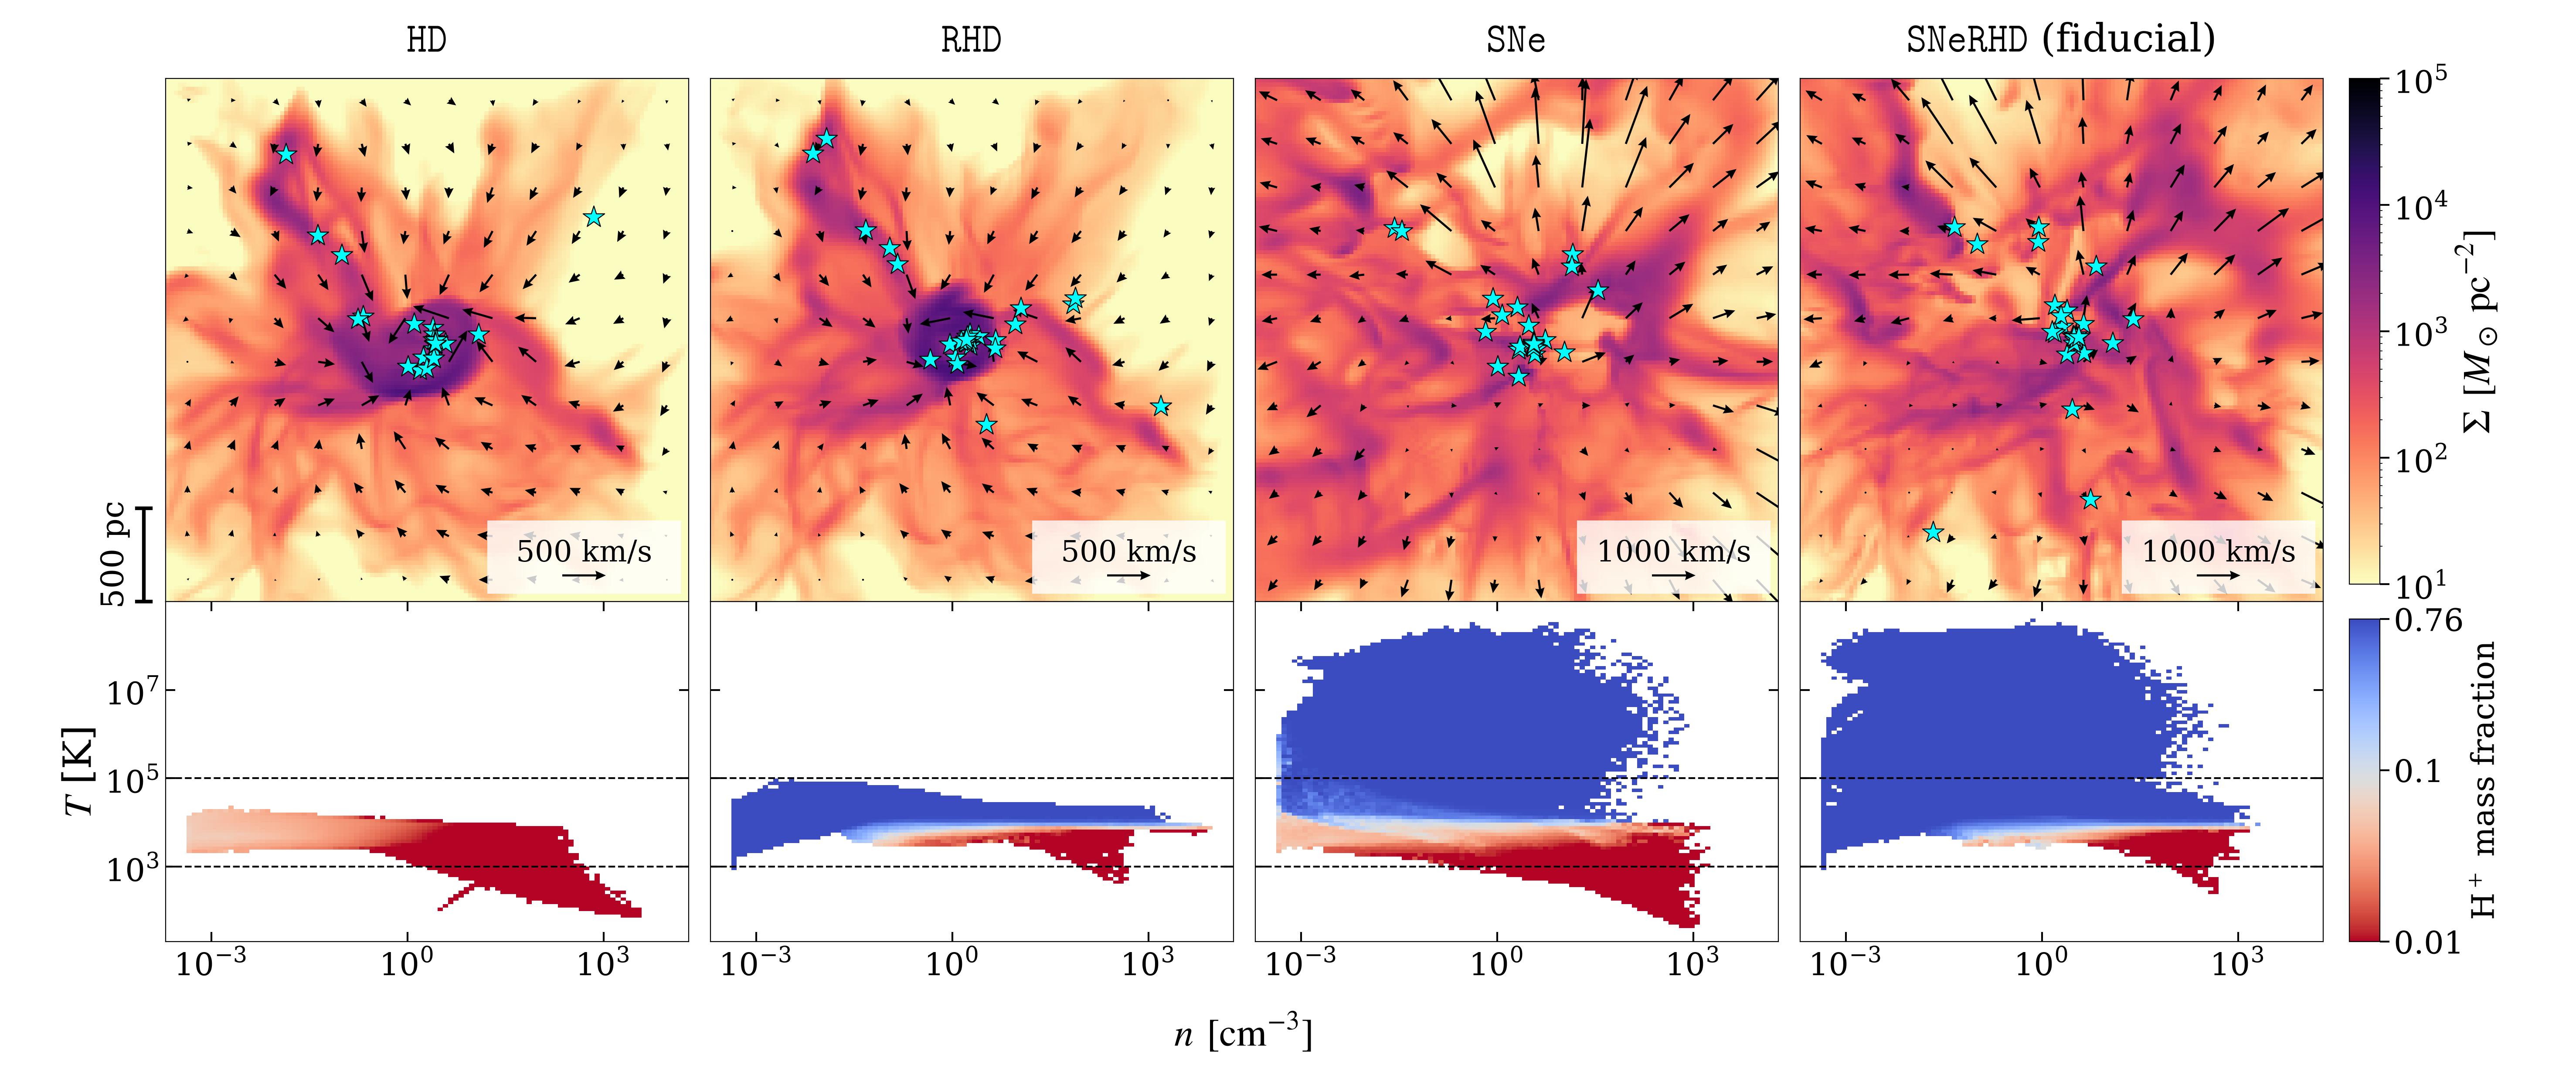
\includegraphics[width=\linewidth]{fig4_snapshots.png}
    \caption{The $\mathtt{HD}$, $\mathtt{RHD}$, $\mathtt{SNe}$ and fiducial ($\mathtt{SNeRHD}$) runs at $t \sim 10$ Myr. Top row: projected gas surface density, with the mass-weighted gas velocity shown as arrows (the key in each panel gives that panel's scale) and star clusters marked as cyan stars. Bottom row: the density--temperature phase diagram, colored by the mass-weighted H$^+$ mass fraction; the horizontal dashed lines indicate the demarcation between the cold, warm, and hot phases. In the control ($\mathtt{HD}$) and radiation-only ($\mathtt{RHD}$) runs, the interstellar gas remains dense, gravitationally bound, and with primarily inward flow direction. On the other hand, the gas in the $\mathtt{SNe}$ run has been dispersed by supernovae and is moving radially outward.}
    \label{fig:feedback_snapshots}
\end{figure*}

The fiducial run includes both radiation and supernovae, so on its own it cannot show which of them stops star formation and drives the outflows. To separate their effects, we compare runs with the same initial conditions in which each mechanism is switched on in isolation (Table \ref{tab:tab1}).
Figure \ref{fig:mstar_runs} shows the integrated star formation efficiency (SFE) as a function of time, 
\begin{align}\label{eq1:sfe}
    \epsilon_* \equiv \frac{M_*}{M_{g,0}}
\end{align}
where $M_*$ is the stellar mass, and $M_{g,0}$ is the initial mass of the gas cloud. Independent of feedback physics, the simulation runs reach $\epsilon_* = 0.17$ within one freefall time ($t_\mathrm{ff}=2.5$ Myr), and $\epsilon_* = 0.64-0.65$ by $2t_\mathrm{ff}$.% \textcolor{red}{and there still hasnt been enough time for jets ?}.

$M_*$ increase monotonically in the hydro-only run ($\mathtt{HD}$), ultimately reaching an SFE of $\gtrsim 93\%$. The $\mathtt{RHD}$ run follows a similar trend, reaching an SFE of $\epsilon_* = 0.90 $ by the simulation end at $t = 8t_\mathrm{ff}$. 


Collapse dominates throughout the runtime of the $\mathtt{RHD}$ simulation, leading to the formation of a bound, coherently rotating disk of gas around the star clusters that is morphologically indistinguishable from the gas in the $\mathtt{HD}$ run. The inability of radiation pressure to regulate star formation in clouds with $\Sigma_\mathrm{gas} > \Sigma_\mathrm{crit}$ is consistent with analytical solutions \citep{2010ApJ...710L.142F,2019MNRAS.483.5548G} and cloud-scale RHD simulations \citep{2023MNRAS.521.5160M}.


% \begin{align}
% \frac{F_\mathrm{UV}}{F_\mathrm{grav}} \sim \frac{\epsilon_* M\langle \sfrac{\dot{p}_*}{M_*}\rangle}{\sfrac{GM^2}{R^2}},
% \end{align}

% where $\langle \sfrac{\dot{p}_*}{M_*}\rangle$ is the rate of specific momentum injection by radiation \citep{2019MNRAS.483.5548G}. Neglecting gas self-gravity, the ratio of the gravitational pressure to the Eddington pressure from UV radiation is given by


Similar to the fiducial simulation, the $\mathtt{SNe}$ run stop forming stars after $t = 6.7$ Myr and plateau at $\epsilon_* \sim 75\%$ (Figure \ref{fig:mstar_runs}).

This coincides with the detonation of the first supernovae, which shock the ISM to $T \sim 10^7\ \mathrm{K}$ and ionize it (Figure \ref{fig:feedback_snapshots}). In addition to quenching star formation, the feedback from supernovae is responsible for disrupting the ISM and driving radial outflows (Figure \ref{fig:postage_fbks}). 

Taken together, these results indicate that supernova feedback is the mechanism capable of halting star formation in the dense gas reservoirs of massive ($10^{11} M_\odot$) haloes in the early Universe, and so may help explain how the UV-bright galaxies that motivated this work clear their gas and dust.

\begin{figure*}[ht!]
    \centering
    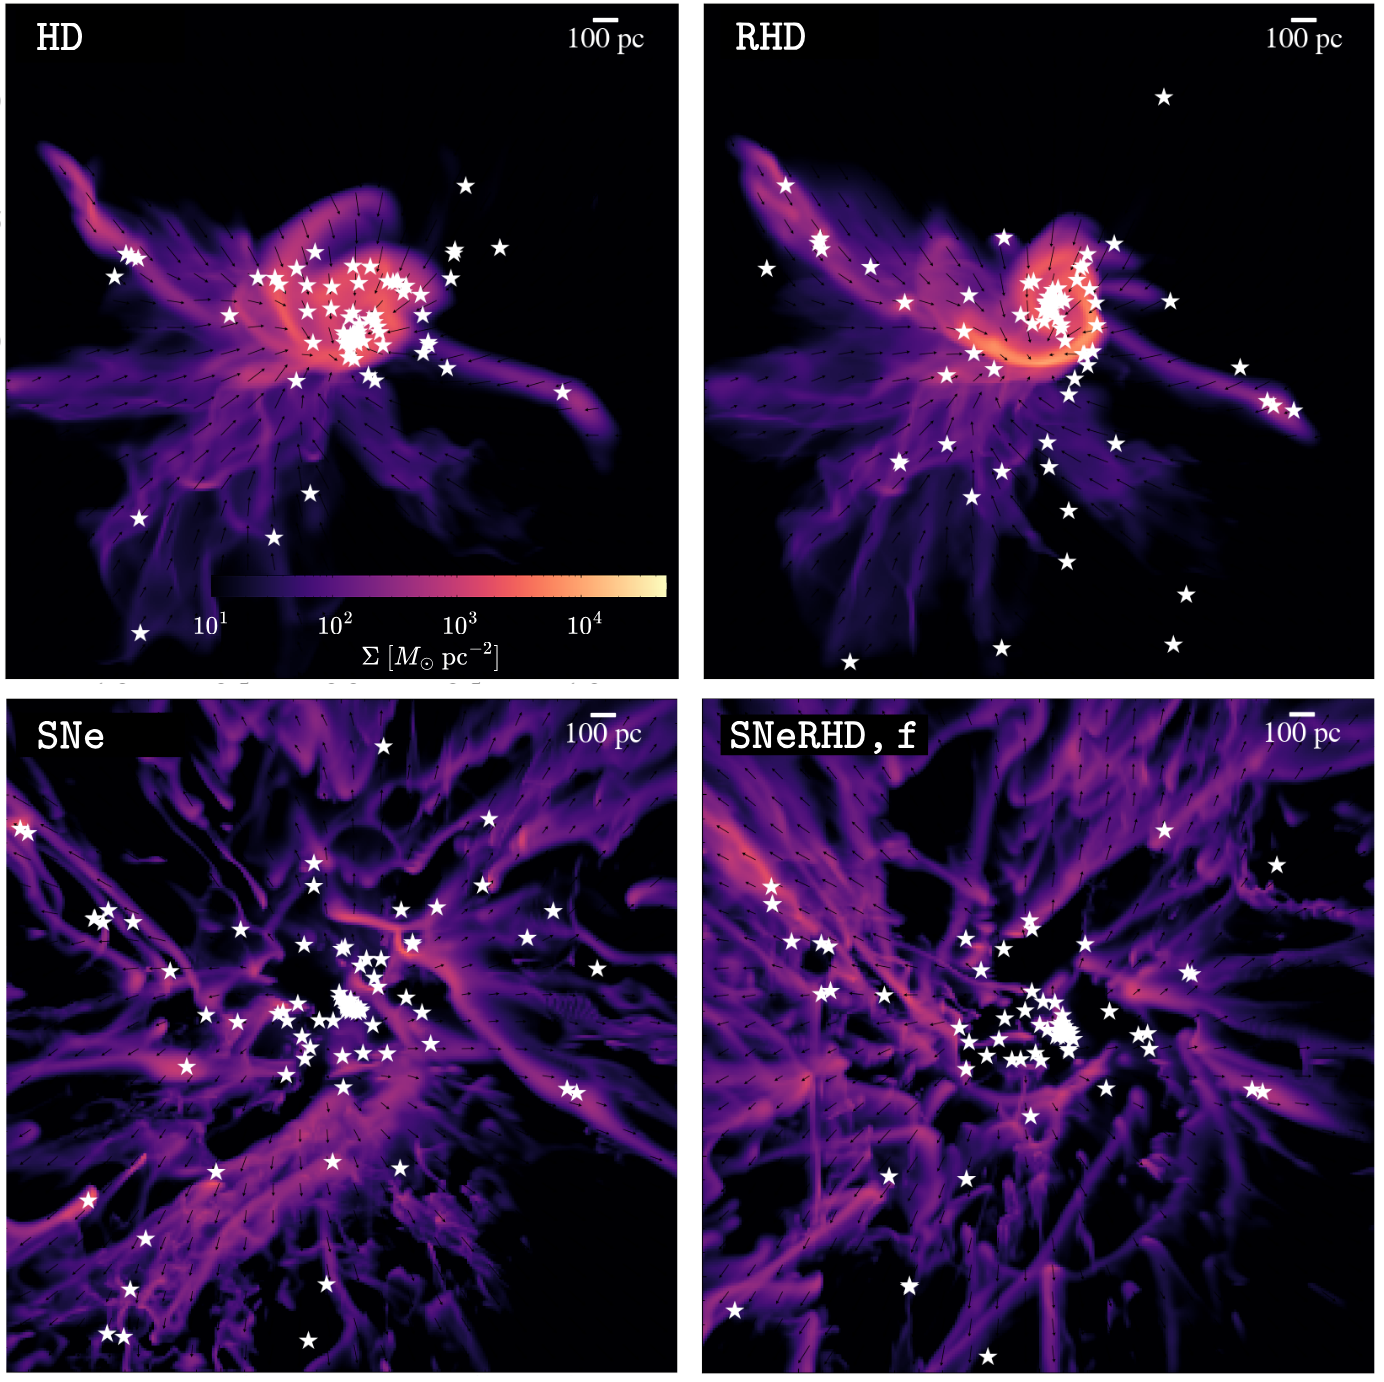
\includegraphics[width=\linewidth]{fig4.png}
    \caption{Left to right: the average outflow velocity averaged between $t_\mathrm{det}$ and $t = 20$ Myr, total mass, momentum and energy carried by the outflows through a spherical surface placed at r = 1 kpc. The error bars on each data point in the velocity panel indicate the 1-$\sigma$ variation of the velocity. The $\mathtt{HD}$ and $\mathtt{RHD}$ runs do not launch an outflow, while the runs with supernova feedback have outflows. The marker colors indicate the phase of the gas, and the grey horizontal lines in the mass, momentum and energy panels show the maximum theoretical yields. 
    % \textcolor{red}{separate by thermal and kinetic energy -- circle vs square, and that will enable separating out what are the radiative energy losses vs kinetic}
}
    \label{fig:phase_diagram}
\end{figure*}

\begin{figure*}[ht!]
    \centering
    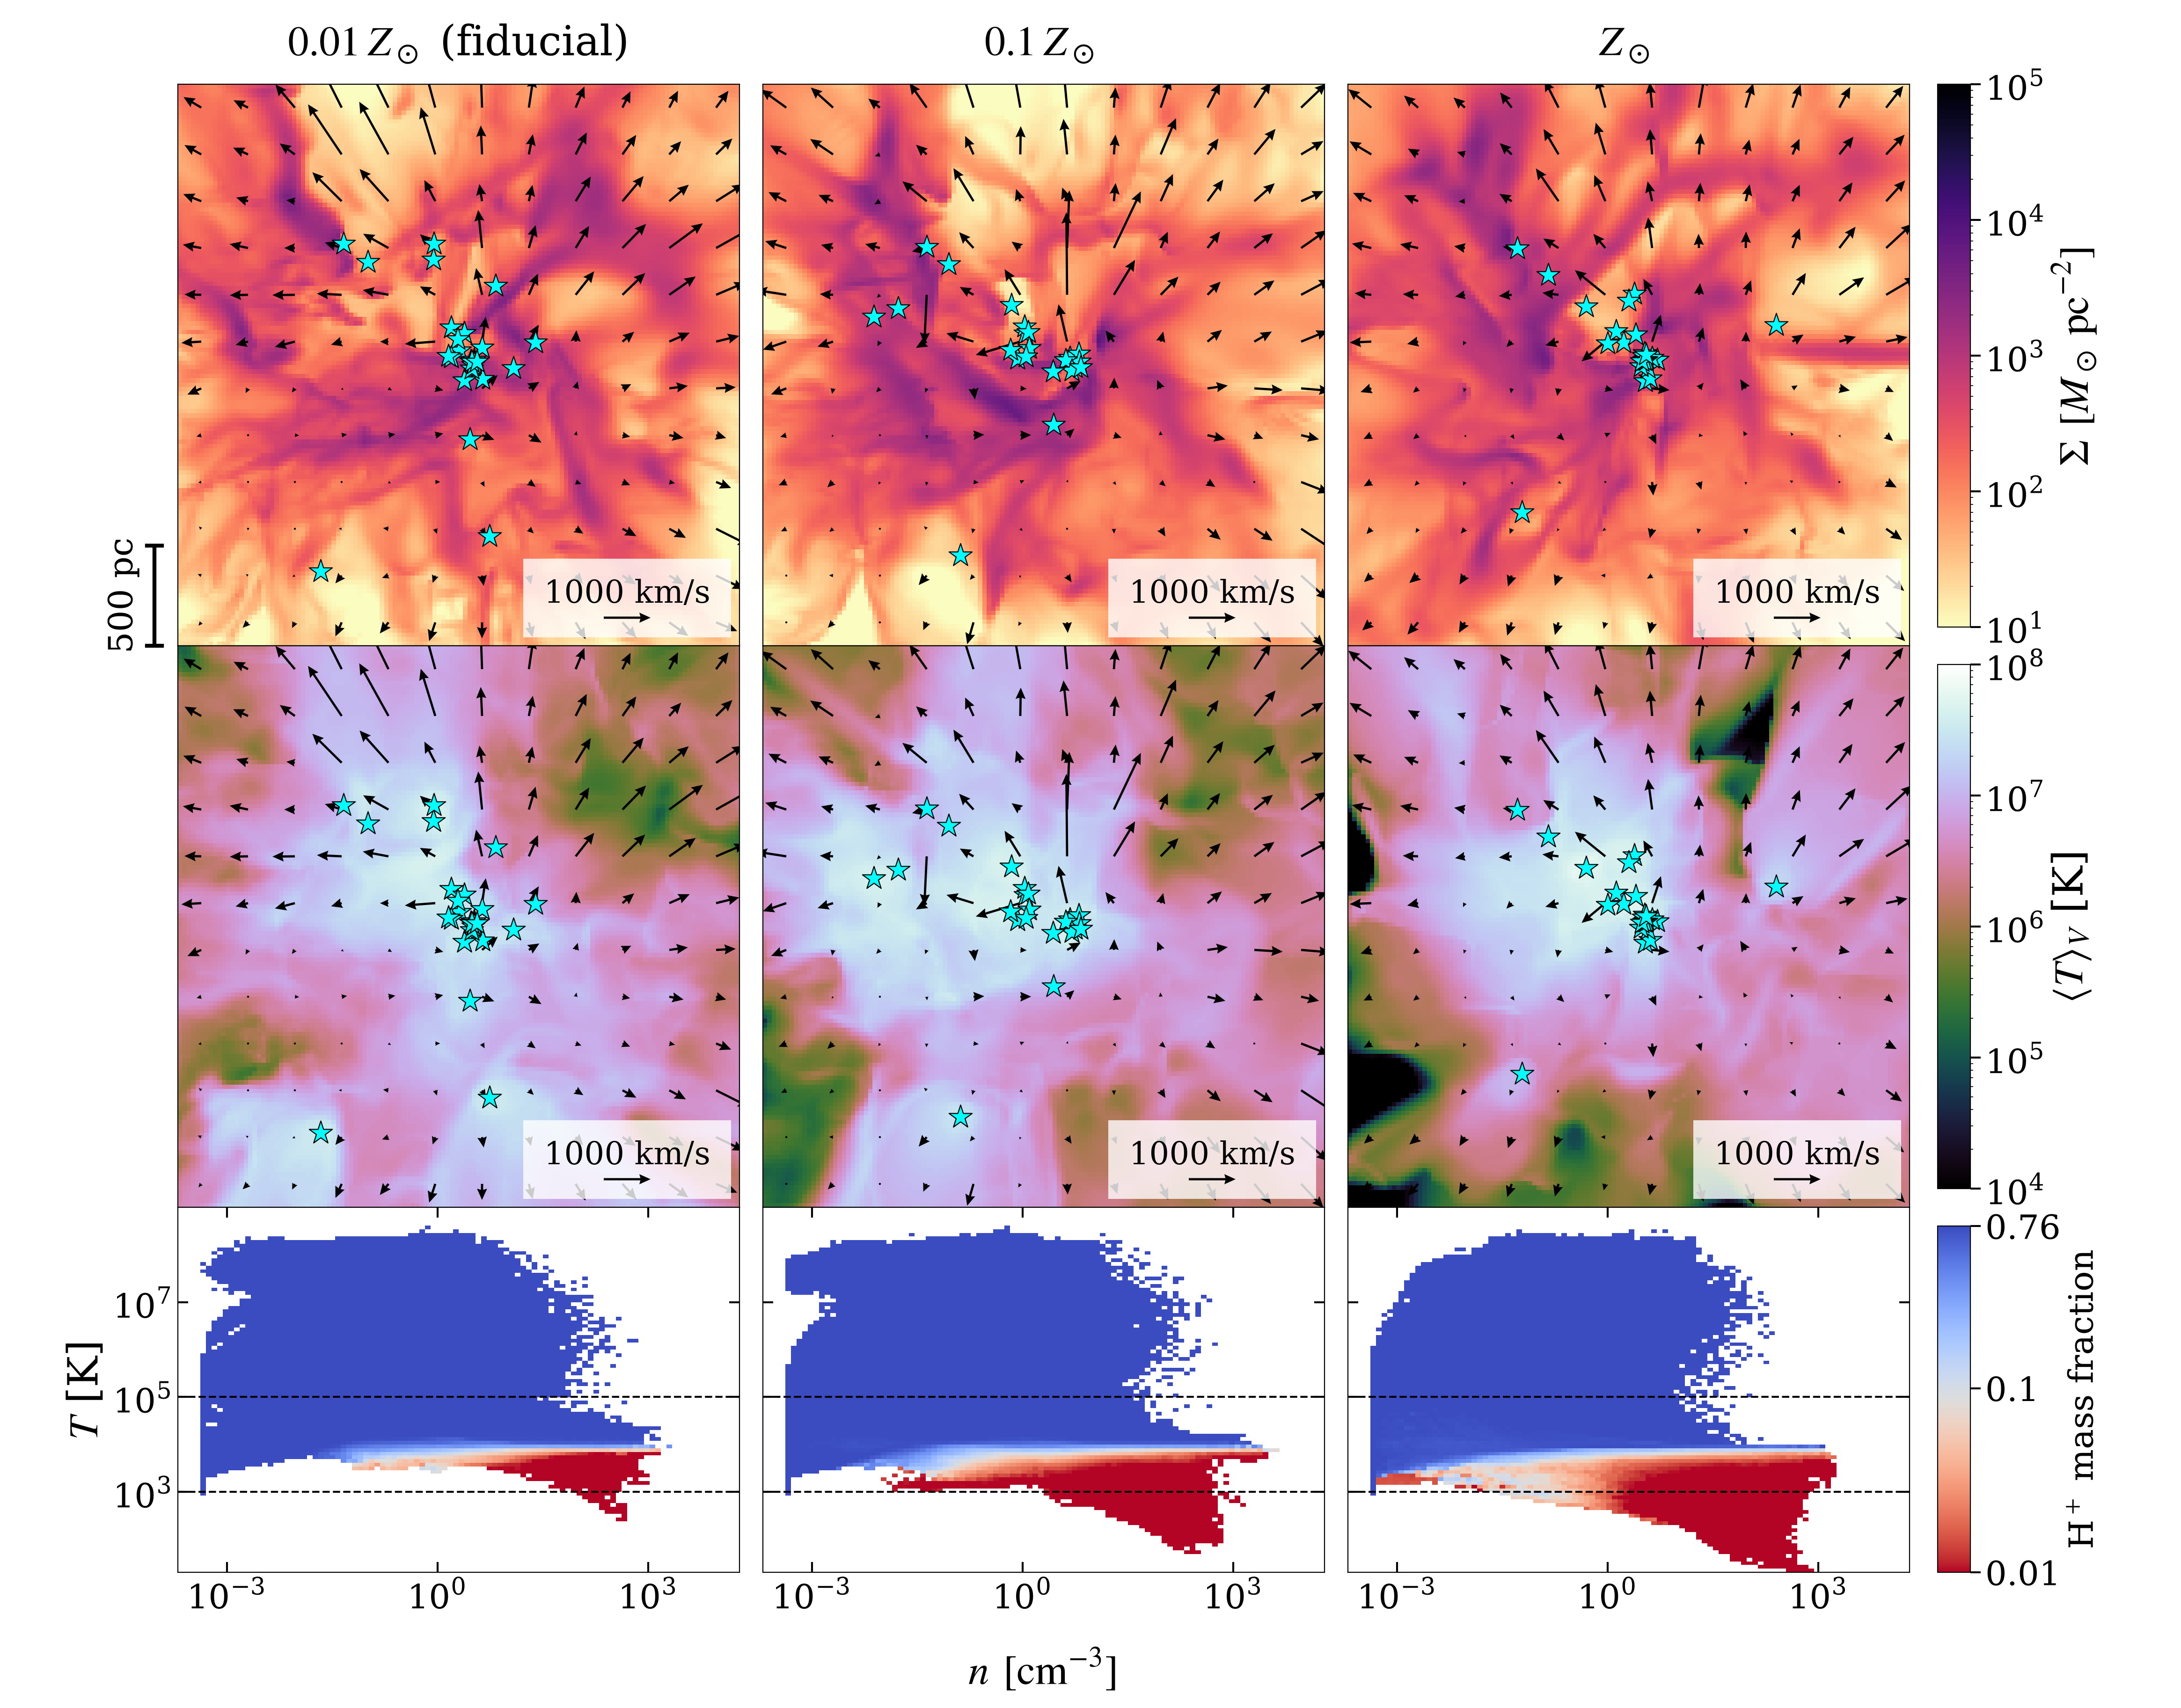
\includegraphics[width=\linewidth]{fig6_snapshots.png}
    \caption{The $\mathtt{SNeRHD}$ runs at $0.01\,Z_\odot$ (fiducial), $0.1\,Z_\odot$ and $Z_\odot$ at $t \sim 10$ Myr. Top row: gas surface density projected along $z$ (the $x$--$y$ plane), with the mass-weighted gas velocity shown as arrows (the key in each panel gives that panel's scale) and star clusters marked as cyan stars. Second row: the volume-averaged temperature along $z$, $\langle T\rangle_V$, with the same velocity arrows and sink particles as the top row. Bottom row: the density--temperature phase diagram, colored by the mass-weighted H$^+$ mass fraction; the horizontal dashed lines indicate the demarcation between the cold, warm, and hot phases.}
    \label{fig:postage_fbks}
\end{figure*}

Star formation histories show that supernovae halt star formation, but not how radiation changes the gas that is expelled. These relative effects become clear when the bulk properties of the outflows are split by thermal phase.


\subsubsection{Phase structure of outflows}
\begin{figure*}[hb!]
    \centering
    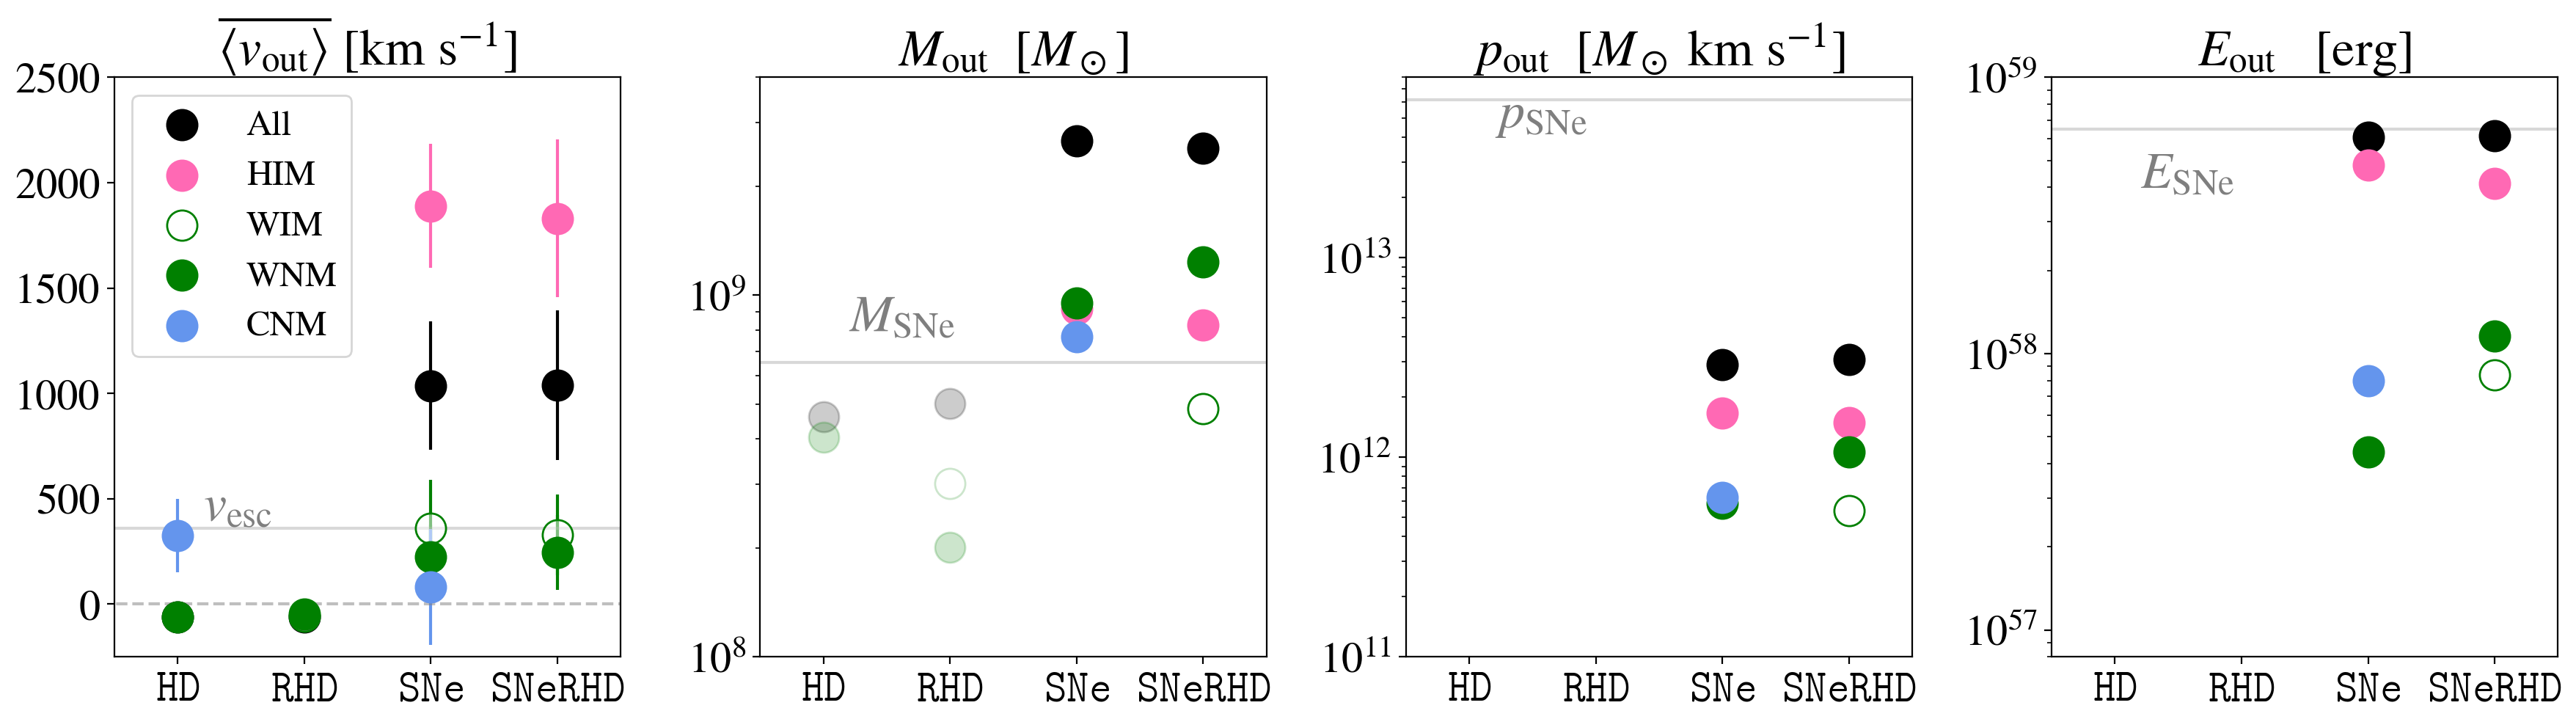
\includegraphics[width=\linewidth]{fig6.png}
    \caption{Bulk properties of the outflows in the $\mathtt{SNeRHD}$ runs at $0.01\,Z_\odot$ (fiducial), $0.1\,Z_\odot$ and $Z_\odot$ (the runs shown in Figure \ref{fig:postage_fbks}), measured through a spherical surface placed at $r = 1$ kpc. Left to right: the time-averaged outflow velocity $\overline{\langle v_\mathrm{out}\rangle}$, and the total mass $M_\mathrm{out}$, momentum $p_\mathrm{out}$ and energy $E_\mathrm{out}$ carried by the outflows between $t_\mathrm{det}$ and $t = 20$ Myr. The marker colors indicate the phase of the gas, as in Figure \ref{fig:phase_diagram}: all gas (black), HIM (pink), WNM (filled green), WIM (open green) and CNM (blue). The error bars in the velocity panel indicate the 1-$\sigma$ variation of the velocity, and the grey horizontal line marks the escape velocity. The grey lines in the mass, momentum and energy panels show the maximum theoretical yields from the supernovae in each run.}
    \label{fig:outflow_phases}
\end{figure*}

The thermal and ionization state of the gas encapsulates information on the impact of the feedback mechanisms, and has direct implications on the observational tracers used to probe the multiphase ISM. In this section we compare the phase structure of the ISM across our simulation suite to quantify these effects (Figure \ref{fig:phase_diagram}). 

We partition the gas into the cold ($T < 10^3\ \mathrm{K}$), hot ($T \geq 10^5\ \mathrm{K}$) and warm phases. While the hot gas is completely ionized and the cold gas is completely neutral, the warm phase is separated into the WNM ($f_\mathrm{ion} < 0.5$) and WIM ($f_\mathrm{ion} \geq 0.5$).

Before examining the outflows themselves, we compare the phase structure of all the gas in the domain across the four physics cases. We do this at $t = 10$ Myr, close to the peak of the supernova rate. At this time, the gas in the $\mathtt{HD}$ run consists of dense CNM ($n > 10^5\ \mathrm{cm^{-3}}$) and WNM at $ \lesssim 10^4$ K covering a wide range of densities $n \in (10^{-1}, 10^5)\ \mathrm{cm^{-3}}$. Due to the UV radiation emitted by the stars, the ISM in the $\mathtt{RHD}$ run is moderately warmer, and significantly ($> 40\%$) ionized. Supernova feedback introduces the HIM, which has $n \in (10^1, 10^3)\ \mathrm{cm^{-3}}$ and makes up $9\%$ of the gas in the simulation at this time. The remaining $91\%$ of the gas is in the warm phases, which is primarily ($55\%$) neutral. 
% On the other hand, there is no cold gas in the $\mathtt{SNeRHD}$ run, and the warm phase is primarily (\textcolor{red}{fraction} ionized).

Figure \ref{fig:outflow_phases} compares the outflows across the four physics cases, showing the average velocity and the total mass, momentum and energy carried through the surface at $r = 1$ kpc by each phase of the gas. In the $\mathtt{HD}$ and $\mathtt{RHD}$ runs, the velocity of the gas is dominated by inflow over the whole course of the simulations. On the other hand, both simulations with supernovae have HIM with average velocities of $1800\ \mathrm{km\ s^{-1}}$ over this same period. The WNM and WIM have outward velocities of $240-330\ \mathrm{km\ s^{-1}}$ ($\sim 0.5 v_\mathrm{esc}$) in $\mathtt{SNe}$ and $\mathtt{SNeRHD}$ runs.

The total gas mass transported by the outflows over the course of the simulation is: 
\begin{equation}
    M_\mathrm{out} = \int_{t=6.7\ \mathrm{Myr}}^{20} \dot{M}_\mathrm{out} \Delta t
\end{equation}
 Integrating $\dot{M}_\mathrm{out}$ over this period, $M_\mathrm{out}$ is approximately equal for the $\mathtt{SNe}$ and $\mathtt{SNeRHD}$ runs, at $\sim 2.5\times 10^9\ M_\odot$. However, the partitioning of this total mass between the phases is different. There is no WIM without radiation, and the $\mathtt{SNe}$ outflows are made up of equal amounts of HIM and WNM ($\sim 10^9\ M_\odot$), with appreciable CNM ($8\times 10^8 M_\odot$). By contrast, in $\mathtt{SNeRHD}$, there is more mass in the WNM ($1.12\times 10^9$), negligible amounts of CNM, and the WIM ($5 \times 10^8 M_\odot$) in $\mathtt{SNeRHD,f}$ now makes up about $30\%$ of the total gas in the warm phase, consistent with our interpretation in Section \ref{sec:bulk} that the winds are energy-driven \textcolor{magenta}{does the WIM fraction really support the energy-driven interpretation?}. There is about the same amount of HIM ($8.3\times 10^8 M_\odot$) as in $\mathtt{SNe}$, which is reflective of the similar rate of supernovae between the two runs.

While the HIM carries only about $30\%$ of the total outflow mass in both runs $\mathtt{SNe}$ and $\mathtt{SNeRHD}$, it dominates the momentum and energy budget of the outflows due to its extreme velocities. 
% The hot winds in the $\mathtt{SNe}$ ($\mathtt{SNeRHD}$) run make up \textcolor{red}{$\gtrsim 60\%$ ($\gtrsim 60\%$)} of the total energy in the outflows. 
% \textcolor{red}{in the sne run, the energy is primarily kinetic? , while in the snerhd it is thermal?}.
This demonstrates that the supernova-driven winds are unable to radiate away thermal energy before they reach the surface at $\sim 1\ \mathrm{kpc}$.
% \textcolor{red}{why does the cnm overtake the wnm in p and e when it has smaller v and m?}
% \textcolor{red}{We also look at the fluxes through a surface at the edge of the simulation, r = 1.4kpc, and the energy is still dominated by thermal /  all the numbers are the same??}
The ability of gas to cool effectively is strongly sensitive to its metallicity, line cooling drives radiative losses at temperatures of $T\ \in (10^5,\ 10^7)\ \mathrm{K}$. In the following section, we discuss how the bulk outflow properties depend on gas metallicity.


\subsection{Photon escape fractions}
\begin{figure*}
    \centering
    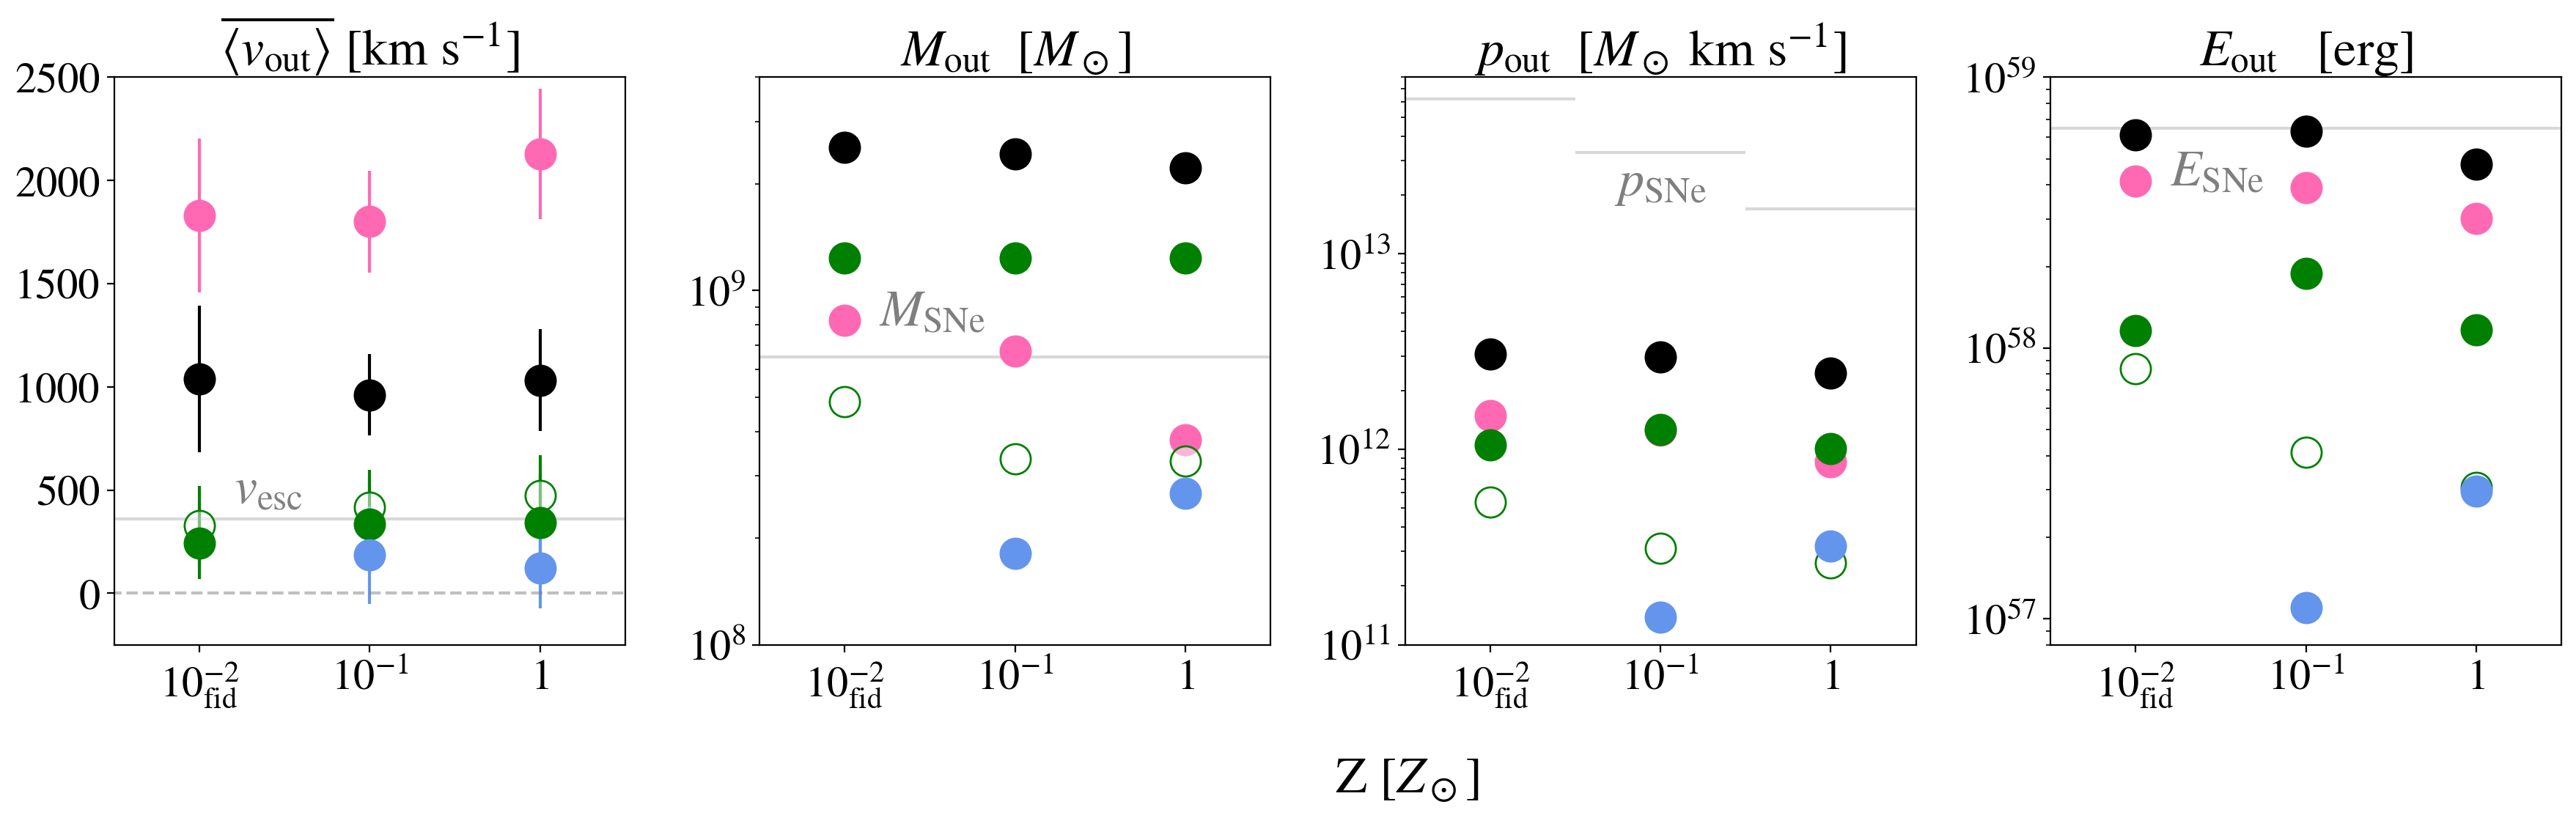
\includegraphics[width=\linewidth]{fig7.png}
    \caption{Escape fraction, $f_\mathrm{esc}$ of photons in the EUV (left), Lyman Werner (middle) and photoelectric (right) bands, for the runs with radiation feedback. The color of the lines indicates feedback physics, and the line style  encodes the metallicity: the fiducial metallicity is $Z = 0.01\,Z_\odot$, which is also the metallicity of the $\mathtt{RHD}$ run. $f_\mathrm{esc}$ is systematically higher in the lower energy bands and shows a strong dependence on metallicity. The presence of supernovae boosts the escape fraction.}
    \label{fig:fesc}
\end{figure*}
% The rest-frame UV luminosity of a starburst galaxy, as well as its capacity to ionize the surrounding intergalactic medium, depends on 
As the interstellar gas and dust are dispersed by supernova-feedback, the fraction of radiation that escapes the system, $f_\mathrm{esc}$, increases with time (Figure \ref{fig:fesc}). $f_\mathrm{esc}$ depends on the relative rates of absorption and emission of UV photons, given by: 
\begin{align}
    f_\mathrm{esc,\nu} = 1 - \frac{\sum (\dot{E}_\mathrm{dust,\nu} + \dot{E}_\mathrm{gas,\nu})dV}{\sum_* L_{*,\nu}}.
\end{align}
The subscript $\nu$ denotes a frequency band, and $L_{*,\nu}$ is the total luminosity of the stellar population in that band. The radiation absorbed by gas and dust is $\dot{E}_{x,\nu} = \kappa_{x,\nu} \rho c E_{r,\nu}$. The dust opacities $\kappa_{\mathrm{dust},\nu}$ are taken from \citet{2011ApJ...732..100D}, while the gas opacity comes from the cross-section of hydrogen to Lyman continuum photons, and is zero in the other bands.

We calculate $f_\mathrm{esc}$ in three frequency bands: extreme UV (EUV), Lyman-Werner (LW) and photoelectric (PE). EUV photons, with energies above $13.6\ \mathrm{eV}$, are absorbed by and ionize neutral hydrogen (HI). LW radiation, with energies $h\nu \in (11.2,13.6)\ \mathrm{eV}$, is absorbed by and dissociates molecular hydrogen, while the PE band, $h\nu \in (6,11.2)\ \mathrm{eV}$, is primarily absorbed by dust grains. 

In the $\mathtt{SNeRHD,f}$ run, LW and PE radiation begin escaping the system immediately upon the formation of the first star clusters, reaching $f_\mathrm{esc} \sim 30\%$ by $t_\mathrm{det}$ (Figure \ref{fig:fesc}). This is shown in the sharp increase of $f_\mathrm{esc}$ in the $\mathtt{SNeRHD}$ run coincident with the onset of the first supernova explosions. After supernovae have been detonating for $\sim 5$ Myr, the escape fraction of LW (PE) photons has risen to $75\%$ ($80\%$). The $f_\mathrm{esc,EUV}$ rises more gradually compared to the other two bands, as the radiation must first ionize the surrounding HI before the system becomes transparent to EUV photons. 

The effect of supernovae on the escape fraction is most pronounced at the lowest metallicity, where approximately $80\%$ of EUV photons, and $\gtrsim 95\%$ of LW and PE escape the system by t = 20 Myr. At higher metallicities, the increased dust content of the ISM leads to more absorption of photons across all three bands, with $3$ (7) times less PE (EUV) radiation leaving the $Z=Z_\odot$ compared to the fiducial metallicity run. This is primarily because of the enhanced attenuation of PE photons by dust and the absorption of EUV and LW photons by the larger column densities of neutral gas.

Since most of the ionizing photons leave the system once the gas has been cleared, the starburst also affects the gas beyond the galaxy. As these photons propagate into the neutral IGM, an ionized bubble forms with a radius of:
\begin{align}
    R_\mathrm{ion} = \left(\frac{3Q_*}{4\pi n_z^2 \alpha_B}\right)^{1/3},
\end{align}

where $Q_*$ is the amount of ionizing radiation emitted by the stellar population, and $\alpha_B = 2.6\times10^{-13}\ \mathrm{cm^3\ s^{-1}}$ is the HI case-B recombination rate coefficient at T = $10^4$ K. The average hydrogen number density of the IGM at redshift $z$ is
\begin{align}
    \bar{n}_\mathrm{H}(z) = \frac{X_\mathrm{H} \Omega_b \rho_{c,0} (1+z)^3}{m_\mathrm{H}} = \frac{3 X_\mathrm{H} \Omega_b H_0^2 (1+z)^3}{8\pi G m_\mathrm{H}},
\end{align}
where $\rho_{c,0}$ is the critical density today. For a $\Lambda$CDM universe with $\Omega_b = 0.049$, $H_0 = 70\ \mathrm{km\ s^{-1}\ Mpc^{-1}}$ and $X_\mathrm{H} = 0.76$, we get $n_z = \bar{n}_\mathrm{H}(10) = 2.7\times 10^{-4}\ \mathrm{cm^{-3}}$. We use $\Omega_b$ rather than $\Omega_m$ here because $n_z$ is the number density of baryonic hydrogen available to be ionized; dark matter does not contribute. Since $\rho_c(z) \approx \Omega_m \rho_{c,0}(1+z)^3$ at these redshifts, $n_z$ is related to the critical density $\rho_c(z)$ used for the NFW halo below (Section \ref{sec:rainback}) by $n_z \approx (\Omega_b/\Omega_m)(X_\mathrm{H}/m_\mathrm{H})\,\rho_c(z)$, i.e.\ the two differ by the cosmic baryon fraction.
The total amount of ionizing photons, $Q_*$ is calculated from the amount of radiation escaping the system:
\begin{align}
Q_* &= \frac{f_\mathrm{esc}L_\mathrm{EUV}}{\langle h\nu \rangle}, 
\end{align}
where $f_\mathrm{esc}$ and $L_\mathrm{EUV}$ are directly measured from the simulations, and we adopt the average photon energy $\langle h\nu \rangle = 18 \mathrm{eV}$ used for our LyC band \citep{2025ApJ...987...12M}.

The sum of UV radiation escaping the starburst in $\mathtt{SNeRHD}$ produces an ionized bubble radius of approximately $11.3\ \mathrm{Mpc}$. Due to their lower $f_\mathrm{esc}$, the higher metallicity runs create smaller bubbles of $7.7\ \mathrm{Mpc}$ and $4.0\ \mathrm{Mpc}$ respectively.
% \textcolor{green}{what is the half-light radius of the system}
A single UV-bright starburst of this kind would therefore ionize a Mpc-scale region of the IGM on its own, comparable to the characteristic $\sim10$ comoving Mpc bubble sizes found around bright sources near the end of reionization in radiative-transfer simulations of the THESAN suite \citep{2025MNRAS.541.1088J,Neyer2026OJAp}. This comparison should be read loosely: those bubble sizes come from full population-level radiative-transfer simulations in comoving units, whereas ours is a single-source, analytic Str\"omgren-sphere estimate in physical units, so the agreement is at most order-of-magnitude and a more careful like-for-like comparison remains to be done. If the UV-bright galaxies observed by JWST at Cosmic Dawn go through a similar phase of feedback-driven gas clearing, they would be efficient sources of ionizing photons, and could contribute substantially to reionizing their surroundings. \textcolor{magenta}{decide: the equilibrium Str\"omgren formula may not apply, since $1/(\alpha_B n) \sim 450$ Myr at the IGM density is far longer than the 20 Myr run. Use a photon-counting radius instead?}
% \textcolor{red}{is this something observable / that people have looked at?}

% \citep{2020MNRAS.499.1395M} measure $R_{ion}$ and find
% \textcolor{red}{This ionized region would extend x of the distance to the nearest other galaxy of comparable size / luminosity. -> any other implications for reionization?} %given the (where does the uvlf = 1)  comoving number density of galaxies at z=10, this is () the average distance between them.

% 1/(alpha * n) is the recombination timescale, calculate and say in words

\subsection{Outflow properties as a function of metallicity}
\begin{figure}[h!]
    \centering
    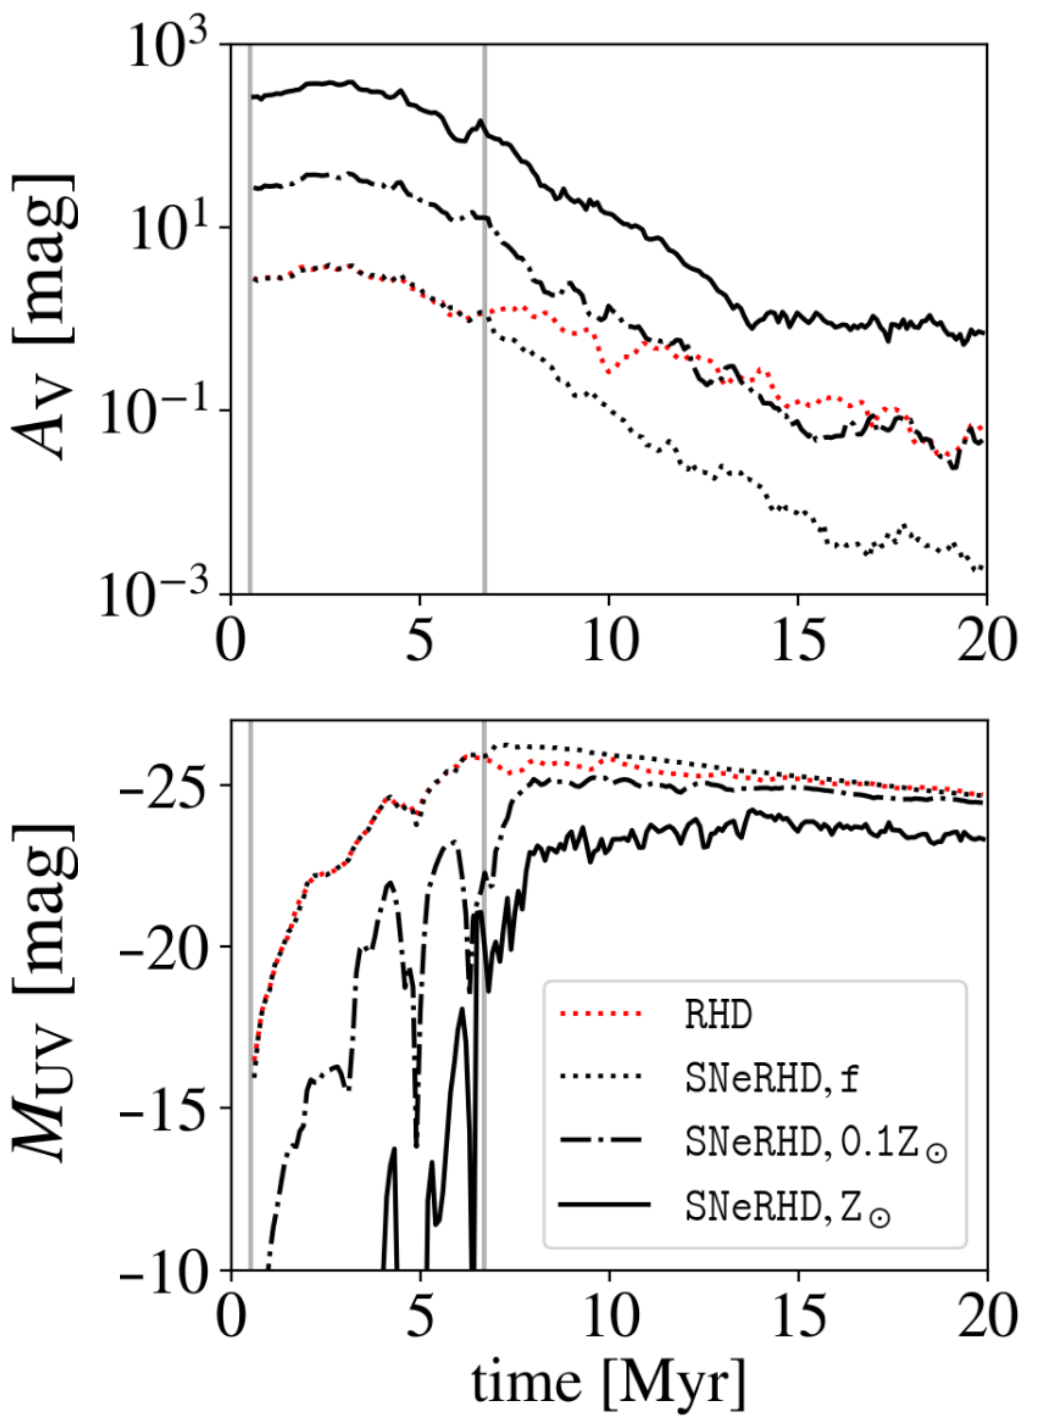
\includegraphics[width=\linewidth]{fig8_stacked.png}
    \caption{Visual-band extinction of the system, $A_\mathrm{V}$ (top) and rest-frame absolute UV magnitude, $M_\mathrm{UV}$ (bottom) for the same simulations shown in Figure \ref{fig:fesc}. The black lines are runs with both supernova and radiation feedback, while the red line is just RHD. The linestyles show the different metallicities of the gas}
    \label{fig:av_muv}
\end{figure}

So far we have considered a system characteristic of the early universe, with a metallicity of $0.01 Z_\odot$. The primary difference in present-day conditions is a higher metallicity, and therefore a higher dust content, which affects both the thermodynamics of the outflows and how visible the system is. Below, we examine how the thermal structure of the outflows changes when the metallicity of the gas is increased by a factor of 10 and 100 in the $\mathtt{SNeRHD,0.1Z}_\odot$ and $\mathtt{SNeRHD,Z}_\odot$ runs, respectively. In Figure \ref{fig:outflow_phases} we compare the bulk properties of the outflows--$\overline{\langle v_\mathrm{out} \rangle}$,$M_\mathrm{out}$, $p_\mathrm{out}$, $E_\mathrm{out}$-- (defined in Section \ref{sec:bulk}) in the $\mathtt{SNeRHD,f}$, $\mathtt{SNeRHD,0.1Z}_\odot$, and $\mathtt{SNeRHD,Z}_\odot$ runs. 

The total mass carried out remains broadly similar across the three metallicities, at $\sim 2\times 10^9 M_\odot$, as does the fraction of the $M_\mathrm{out}$ residing in the WNM. On the other hand, there is a systematic decrease in the HIM, with the outflow mass in the HIM being $20\%$ less in the $\mathtt{SNeRHD,0.1Z}_\odot$, and half in the  $\mathtt{SNeRHD,Z}_\odot$, in comparison to the fiducial run. The WIM also decreases, albeit moderately, by $\sim 30\%$ to $\approx 3\times10^8M_\odot$ in the higher metallicity runs. Correspondingly, the CNM now makes $8\%$ ($10\%$) of the wind mass at $Z=0.1Z_\odot$ ($Z=Z_\odot$). Since the total mass stays roughly constant, these trends imply that the outflowing mass shifts from the hot phase into cooler phases as the metallicity increases. \textcolor{magenta}{confirm this interpretation}

The outflow velocity averaged over the winds is broadly consistent across $\mathtt{SNeRHD,f}$,$\mathtt{SNeRHD,0.1Z}_\odot$, and $\mathtt{SNeRHD,Z}_\odot$, as is the relative speeds of the warm and hot phases. The velocity of the HIM increases moderately with metallicity, reaching $2100\ \mathrm{km\ s^{-1}}$ in the $\mathtt{SNeRHD,Z}_\odot$ run. Both warm phases also speed up with Z, with a $40\%$ increase in $\langle v \rangle$ from the fiducial metallicity to solar. The CNM, which was predominantly inflowing in $\mathtt{SNeRHD,f}$, is now part of the outflow, as more of the outflowing hot material cools onto cooler gas and/or is entrained in the outflow. 
% \textcolor{red}{with velocities of $number \mathrm{km\ s^{-1}}$ at 0.1 zsun and zun.}

The partition of momentum and energy between the phases reflects the competing effects of the trends in mass and velocity. The total momentum is $p_\mathrm{out} \sim 3\times10^{12}\ M_\odot \mathrm{km\ s^{-1}}$ across the three runs. $p_\mathrm{out,HIM}$ decreases by about $40\%$ from $0.01Z_\odot$ to solar metallicity, accompanied by an increase in the fraction of the total momentum residing in the WNM and CNM phases, which follows from the shift in mass out of the hot phase. 
% \textcolor{red}{much more radial momentum is conserved because the ejecta are cooling adiabatically?}

The total energy carried by the outflows also decreases with Z---while the $\mathtt{SNeRHD,f}$ and $\mathtt{SNeRHD,0.1Z}_\odot$ runs are energy conserving ($E_\mathrm{out}\sim N_\mathrm{SNe} \times 10^{51}\ \mathrm{erg}$), the energy of the winds at solar metallicity is $E_\mathrm{out}(Z_\odot) \sim 0.7 N_\mathrm{SNe} \times 10^{51}\ \mathrm{erg}$. This indicating that ISM gas in conditions more similar to the local universe radiatively cools more effectively. The low metal and dust abundances at the fiducial metallicity ($0.01Z_\odot$) limit the radiative cooling efficiency of the hot gas in the $\mathtt{SNeRHD,f}$ run.


% \newpage


\section{Discussion}
The overabundance of UV-bright galaxies at Cosmic Dawn has motivated analytical models in which these systems form stars efficiently and then lose their gas and dust to feedback. Our simulations test this sequence directly: the fiducial run reaches $\epsilon_* \sim 0.76$ before supernovae clear the ISM, after which $\gtrsim 80\%$ of the UV photons escape the system. Below, we compare these results to observations, analytical models and other simulations.
\subsection{Comparison with observations}

\begin{figure}%[ht!]
    \centering
    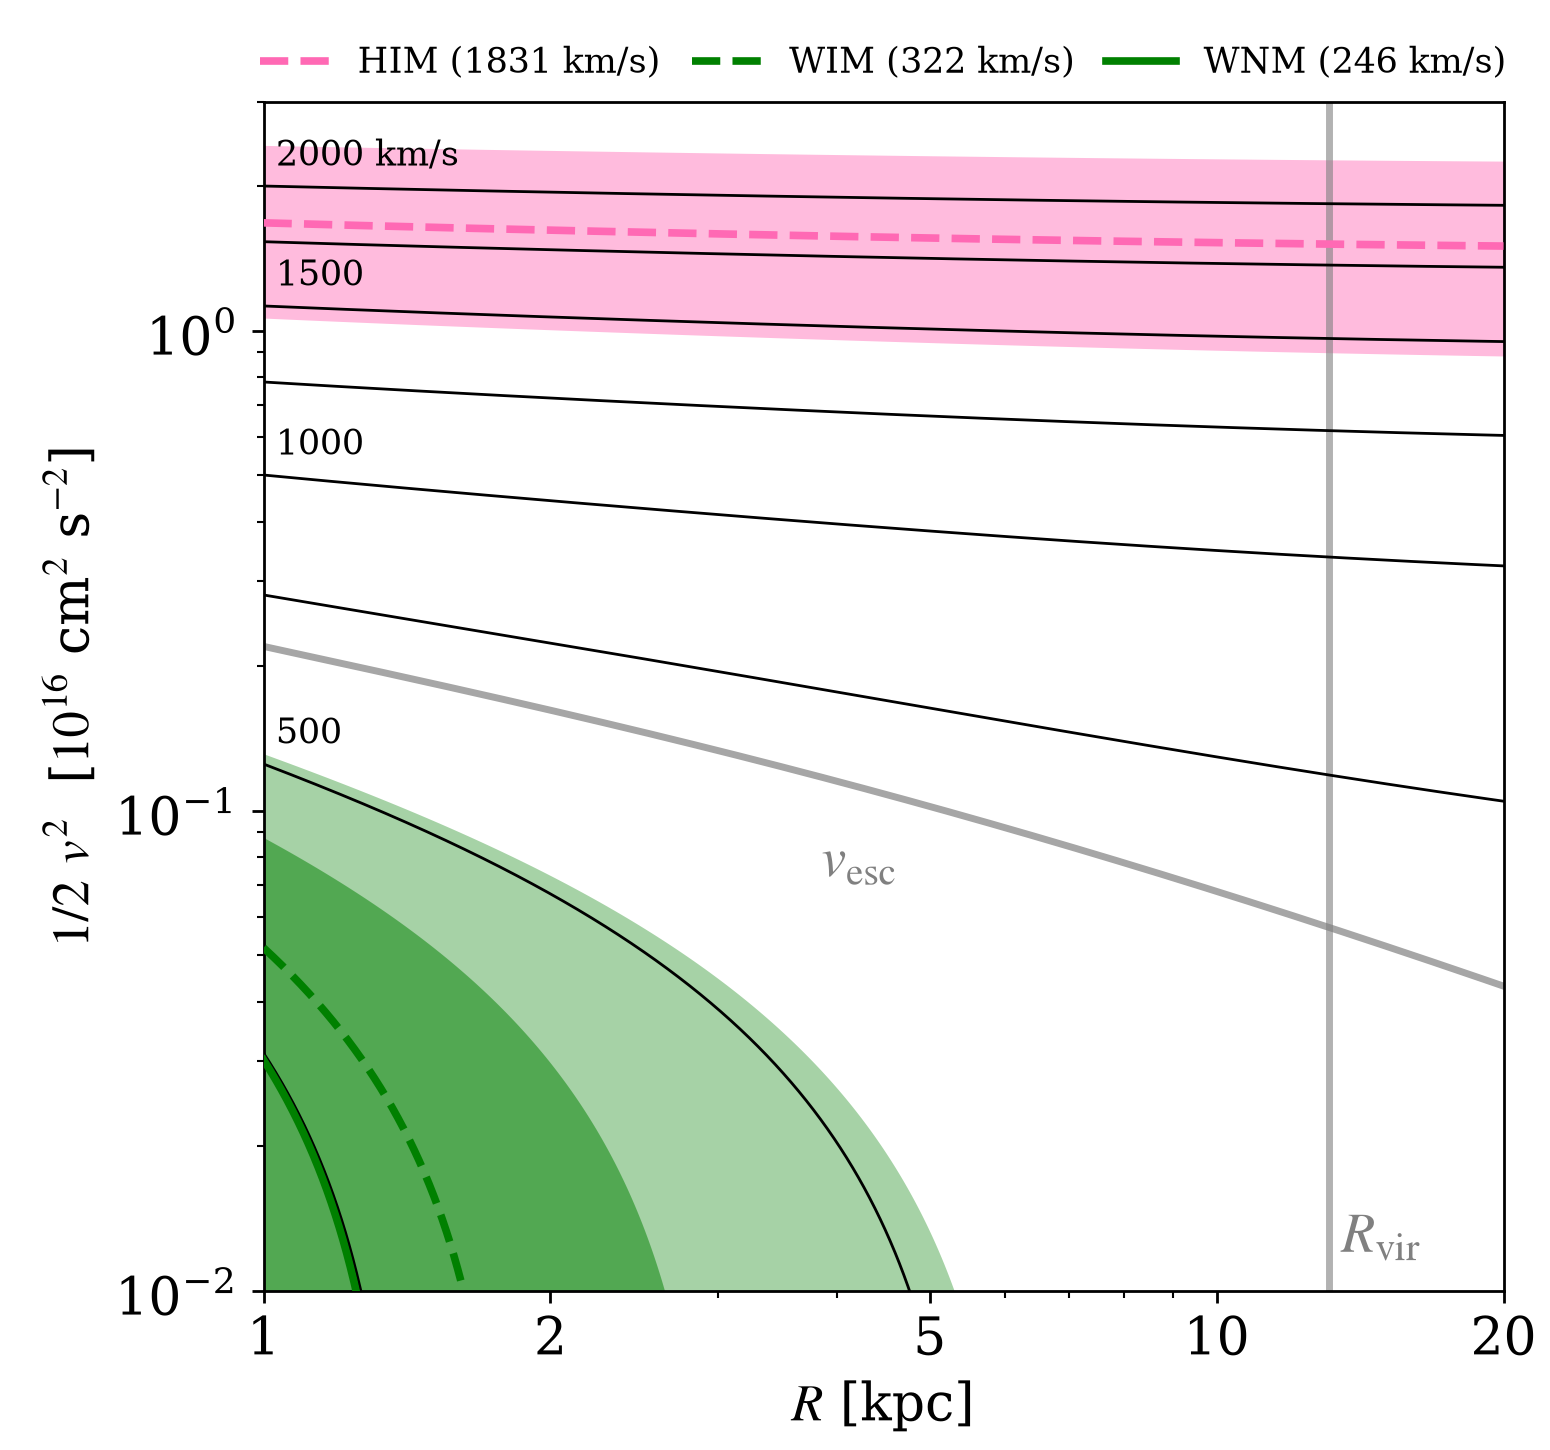
\includegraphics[width=\linewidth]{fig10_ekin.png}
    \caption{Specific kinetic energy, $\frac{1}{2}v^2 = e_\mathrm{init} - \Phi(R)$, of gas launched from $R_\mathrm{launch} = 1$ kpc as it moves out through the potential of the starburst and its dark matter halo. Black lines are trajectories labelled by their launch velocity; the grey curve is the escape trajectory ($e_\mathrm{init} = 0$), and the vertical line marks the virial radius. The colored lines show the outflow phases of the fiducial simulation, launched at the median of $\langle v_\mathrm{out}\rangle$ over $6.7-20$ Myr (dashed pink: HIM; dashed green: WIM; solid green: WNM), and the shaded regions span $\pm 1\sigma$ of the velocity over the same period. Bound gas reaches $R_\mathrm{max}$ where its curve drops to zero.}
    \label{fig:etot}
\end{figure}

The rest-frame UV magnitude of the fiducial run follows the eras described in Section 3.1 (Figure \ref{fig:av_muv}). During gravitational collapse, $M_\mathrm{UV}$ brightens rapidly as stars form, from $\approx -16$ mag at 0.5 Myr to $\approx -22$ mag by 2 Myr. It peaks near $M_\mathrm{UV} = -26$ mag at $\sim 7$ Myr, just after the first supernovae detonate, and then fades slowly during the dispersal era as the stars age and die, to $M_\mathrm{UV} \approx -25$ mag at $t = 20$ Myr.
% \textcolor{red}{(maybe make a figure compiling literature?)}


The massive galaxies observed by JWST at Cosmic Dawn have typical rest-frame UV magnitudes of $\sim -20\ \mathrm{mag}$ (e.g, \citealt{2024A&A...691A..87M}), so at $t = 20$ Myr the simulated starburst is $\sim 5$ mag brighter. This extreme UV brightness is in part a consequence of the large halo mass adopted in this work. \citet{2025MNRAS.543.3802Y} model the star formation efficiency $\epsilon_*(M_\mathrm{halo},z)$ as a function of halo mass within an abundance-matching framework fit to the observed UV luminosity function, from which $M_\mathrm{UV}$ follows via $\mathrm{SFR} = \epsilon_* f_b \dot{M}_\mathrm{halo}$ and a standard UV-to-SFR conversion; their Figure 3 shows that even under this model's most efficient case ($\epsilon_*=1$), a halo as massive as ours at $z\sim16$--20 hosts a galaxy with $M_\mathrm{UV}$ comparable to what we find here.

Comparing the physics cases, the difference between the $\mathtt{RHD}$ and $\mathtt{SNeRHD}$ runs remains $< 0.5\ \mathrm{mag}$ even after the detonation of the first supernovae, indicating that the photoionization is sufficient to allow the escape of UV photons. Both runs become fainter at late times, consistent with the decreased UV output as the stars age and die.

Metallicity has substantial effects on $M_\mathrm{UV}$, especially in the first 5 Myr. The dust-to-gas ratio of the $\mathtt{SNeRHD,0.1Z}_\odot$ and $\mathtt{SNeRHD,Z}_\odot$ runs is a factor of 10 and 100 larger than the fiducial case. This leads to increased absorption of UV photons by dust at higher Z, and the $M_\mathrm{UV}$ remains faint during the gravitational collapse phase. \textcolor{magenta}{needs a quantitative check: the $M_\mathrm{UV}$ data behind Figure \ref{fig:av_muv} are not available locally to confirm a precise average} Visual inspection of Figure \ref{fig:av_muv} suggests the $\mathtt{SNeRHD,0.1Z}_\odot$ run is dimmer than this by more than $\sim3$ mag outside its brief oscillation spikes (closer to $5-8$ mag), while the $Z = Z_\odot$ run is $\gtrsim 10$ mag dimmer. Once the supernovae clear the gas, the higher metallicity runs brighten significantly, reaching $M_\mathrm{UV} \sim -23$ by $t=20$ Myr.

\subsection{Comparison with analytical models}
% \textcolor{limegreen}{(needs to be double-checked) background on the jwst observations and the theoretical models in response -- how to expand this beyond intro? and what portion of the time to tie back vs to talk about "the results we've gotten (mass loading factor etc(and also from before whose results have implications on the physics)}
The UV brightness of the simulated system depends on how much of its dust is cleared, which is the central prediction of analytical models of feedback-driven winds. We estimate the UV continuum slope $\beta_\mathrm{UV}$ (where $f_\lambda \propto \lambda^\beta$) from the simulated visual-band extinction $A_\mathrm{V}$ (Figure \ref{fig:av_muv}) in two steps. First, we convert $A_\mathrm{V}$ to the rest-frame UV attenuation at 1600\,\AA, $A_{1600}$, using the \citet{2000ApJ...533..682C} starburst attenuation curve, $A_{1600}/A_\mathrm{V} \approx 2.55$. We then convert $A_{1600}$ to $\beta_\mathrm{UV}$ using the empirical relation of \citet{1999ApJ...521...64M}, $A_{1600} \approx 4.43 + 1.99\,\beta_\mathrm{UV}$. Both relations are calibrated on local, moderately attenuated UV-selected starbursts and break down once the dust becomes optically thick, so we apply them only once feedback has cleared most of the gas ($t\gtrsim10$ Myr, $A_\mathrm{V}\lesssim0.3$ mag in the fiducial run). Over this period we find $\beta_\mathrm{UV}\approx -1.8$ to $-2.1$; the bluer end of this range falls within the blue colors ($-2.9<\beta_\mathrm{UV}<-2.0$) measured in the JWST-observed blue monsters that motivate this work, while the redder end is somewhat redder than that observed range.
\cite{2023MNRAS.522.3986F} proposed that once high-redshift galaxies cross a sSFR threshold of $25\ \mathrm{Gyr}^{-1}$, super-Eddington winds expel the interstellar dust and gas. In our simulations, we test whether the removal of the ISM by outflows is sufficient to render the young stellar population directly visible in the UV. 

The visual band extinction $A_\mathrm{V}$ in the $\mathtt{RHD}$, $\mathtt{SNeRHD,f}$, $ \mathtt{SNeRHD,0.1Z}_\odot$, and $\mathtt{SNeRHD,Z}_\odot$ runs is shown as a function of time in Figure \ref{fig:av_muv}. We first compare the $\mathtt{RHD}$ and $\mathtt{SNeRHD,f}$ runs, which differ only in the presence of supernovae and so directly test whether feedback-driven outflows clear the dust. During the first 5 Myr, the two runs have the same extinction, $A_\mathrm{V}\sim 3\ \mathrm{mag}$. Once supernovae detonate and begin clearing the gas, $A_\mathrm{V}$ in $\mathtt{SNeRHD,f}$ falls to $\sim 10^{-3}\ \mathrm{mag}$ by $t = 20$ Myr, more than an order of magnitude below the $\mathtt{RHD}$ run ($\sim 0.1\ \mathrm{mag}$), producing an essentially dust-free stellar population. This mechanical clearing is consistent with the dust-blowout picture proposed by \citet{2026A&A...705L..10M}, who show that clustered supernovae in stratified, self-gravitating clouds can mechanically vent most of the dust from young star clusters, predicting retained dust-to-stellar mass ratios in the same range inferred for spectroscopically confirmed blue monsters.

The metallicity of the gas sets the extinction before the supernovae: during the first 5 Myr, the $\mathtt{SNeRHD,0.1Z}_\odot$ ($\mathtt{SNeRHD,Z}_\odot$) run has 10x (100x) higher extinction than the fiducial run, owing to the increased dust abundance in the ISM. Once supernovae detonate, $A_\mathrm{V}$ drops at all metallicities, to $\lesssim 10^{-1}\ \mathrm{mag}$ in the $\mathtt{SNeRHD,0.1Z}_\odot$ run, while the $\mathtt{SNeRHD,Z}_\odot$ run retains $A_\mathrm{V} \sim 0.6\ \mathrm{mag}$ at $t = 20$ Myr.
% This would produce an unattenuated starburst with blue UV slope $\beta_\mathrm{UV} \lesssim -2$, a scenario supported by analytical models of feedback-driven outflows (e.g., \citealt{2024A&A...684A.207F,2023MNRAS.520.2445Z}).
The clearing of the ISM by supernovae produces correspondingly larger jumps in the UV luminosity, which we discuss in the section below.



\subsection{Comparison with simulations}
Hydrodynamic simulations of conditions emulating both the local and early universe demonstrate that supernovae can drive energetic outflows that efficiently remove gas and dust from galaxies (e.g.,\citealt{2026ApJ..1000..158C,2018MNRAS.481.3325F}).

Cosmological zoom-in simulations provide a numerical counterpart to the set up described here \citep{
2025MNRAS.536..988F,2026arXiv260524104S,2026MNRAS.545f2119S,2025MNRAS.540.3350A}. \cite{2025MNRAS.540.3350A} run a cosmological zoom-in simulation of a halo with the same mass as presented in this work, $10^{11}\ M_\odot$. The galaxy undergoes several episodes of star formation between $z \in (14,\ 9)$, assembling a stellar mass of $3 \times 10^9 M_\odot$ by z = 9. The galaxy has an instantaneous SFR of $30-50\ M_\odot \ \mathrm{yr^{-1}}$, and an integrated SFE of $\epsilon \sim 0.1-0.3$.

The higher SFE in our simulations in comparison to \cite{2025MNRAS.540.3350A} reflects the physical differences of our set-ups. The simulations presented here each represent an isolated cloud, which lacks cosmological accretion history from the intergalactic medium. This new gas would decrease the star formation efficiency by keeping the total gas mass elevated. Additionally, the star formation in this work occurs in a single burst, while in \cite{2025MNRAS.540.3350A}'s case, accretion from the IGM both i) decreases the instantaneous SFE and ii) sustains star formation long-term by supplying fuel. 


\subsection{Outflow rainback time}\label{sec:rainback}

Our simulations end at 20 Myr, while the longer-term evolution of these systems depends on whether the expelled gas escapes or returns to fuel further star formation. Cosmological zoom-in simulations such as those above follow these longer timescales, and work on quenched galaxies at lower redshift suggests that outflows may play a role \citep{2015ARA&A..53...51S,2024ApJ...964...76G}. To connect our results to these timescales, we create a one-dimensional model for how the outflows evolve once they enter the CGM. We take $\langle v\rangle _\mathrm{out}$ averaged over t$ =6.7 - 20$ Myr as the launch velocity, and treat the outflow as a projectile moving through total gravitational potential of the system, $\Phi (r) = \Phi_\mathrm{bary}(r) + \Phi_\mathrm{DM}(r)$. This allows us to estimate the maximum distance that the gas travels to, $R_\mathrm{max}$, before being recycled back onto the system 

The baryonic potential $\Phi_\mathrm{bary}$ is calculated by treating the starburst as a spherically symmetric distribution of $M_* = \epsilon_* M_\mathrm{g,t0}$ with a radius of 500 pc (Figure \ref{fig:mstar_evolution}). The star clusters are centrally concentrated: between 10 and 20 Myr, their half-mass radius is $\lesssim 100$ pc, and more than $90\%$ of the stellar mass lies within $500$ pc. At $r \geq R_\mathrm{launch} = 1$ kpc the starburst therefore acts as a point mass, and the adopted radius does not affect $\Phi_\mathrm{bary}$. The dark matter contribution, $\Phi_\mathrm{DM}$, is modelled as an NFW potential \citep{1997ApJ...490..493N} with a concentration parameter of $c=10$. Our results are relatively insensitive to this choice: for $c = 5-20$, the escape velocity at 1 kpc changes by $\lesssim 6\%$ ($634-702\ \mathrm{km\ s^{-1}}$), and $R_\mathrm{max}$ of the warm phases by $\lesssim 20\%$. 

The total gravitational potential of the system is then: 
\begin{align}
\Phi_\mathrm{tot}(r) = - \frac{G M_*}{r} - \frac{4\pi G \rho_0 R_s^3}{r}\ \ln\left(1 + \frac{r}{R_s}\right),
\end{align}
where $R_s = r_{200}/c = 1.3kpc$ is the scale radius of the dark matter halo, and $\rho_0 = \frac{2}{3}\rho_c(z) \times 10^5 /(\ln 11 - 10/11)$ is its central density.

A gas parcel launched into $\Phi (r)$ with an initial velocity of $v_\mathrm{init} = \langle v_\mathrm{out} \rangle$ will have a total energy of:
\begin{align}
e_\mathrm{init} = \Phi(R_\mathrm{launch}) + \frac{1}{2}v_\mathrm{init}^2.
\end{align}

Figure \ref{fig:outflow_phases} shows that the phases of the outflow have dramatically different launch velocities across all the simulations. In the fiducial run, the HIM is launched with velocity of $1800\ \mathrm{km\ s^{-1}}$ from $R = 1\ \mathrm{kpc}$. Since $\langle v_\mathrm{out} \rangle_\mathrm{HIM}$ is much larger than $v_\mathrm{esc}$, the hot winds permanently escape the system, enriching the IGM.
% with the $M_\mathrm{out,HIM} \times f_d$, where \textcolor{red}{$f_d = number$ is the amount of dust and metals formed in the supernovae. cite someone from foley and co}. 

\begin{figure}[ht!]
    \centering
    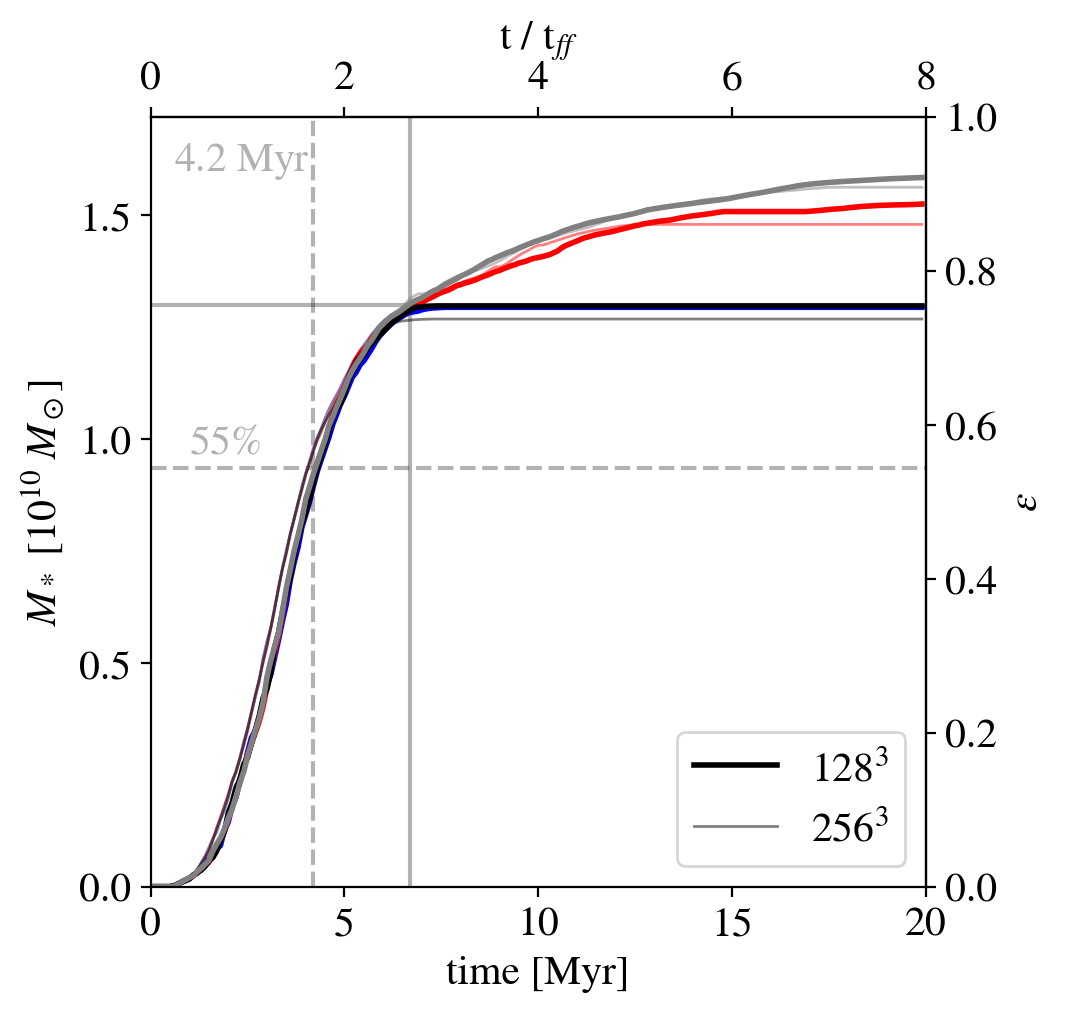
\includegraphics[width=\linewidth]{fig10.png}
    \caption{Stellar mass formed in the simulations as a function of resolution. The line color indicates the feedback physics, and the thickness encodes the resolution of each run. Across all four physics cases, the star formation efficiency is consistent across the resolutions, indicating that the simulations are numerically converged.}
    \label{fig:resolution}
\end{figure}

The WNM and WIM, on the other hand, remain bound, since their launch velocities, $240\ \mathrm{km\ s^{-1}}$ and $330\ \mathrm{km\ s^{-1}}$, are well below $v_\mathrm{esc}$. To calculate the maximum radius $R_\mathrm{max}$ that warm gas reaches before being raining back onto the galaxy, we compute the maximum radius from the conservation of total energy of the system, defining this point to be where the kinetic energy of the gas drops to zero: 
% maximum  remember that winds are energy-conserving and set $e_\mathrm{init}(r) = e_\mathrm{tot}(R_\mathrm{max})$ for all $r$. By the definition of the maximum radius,
\begin{align}
    e_\mathrm{init} - \Phi(R_\mathrm{max}) = 0
\end{align}

Solving the above equation for each phase, we find that the WNM reaches a maximum radius of $\sim 1.4\ \mathrm{kpc}$ before raining back. The WIM is launched at a slightly faster velocity, so it gets to $\sim 2\ \mathrm{kpc}$.

The time it would take for the outflowing gas to return to the launch radius is $t_\mathrm{rain} = 2t_\mathrm{max}$, where $t_\mathrm{max}$ is given by:
\begin{align}
t_\mathrm{max} = \int_{R_\mathrm{launch}}^{R_\mathrm{max}}\sqrt{2(e_\mathrm{tot} - \Phi(r)\bigr)},
\end{align}

The WNM rains back onto the system after $6.1\ \mathrm{Myr}$, while the WIM travels for a total of $11.4\ \mathrm{Myr}$. These numbers are likely upper limits, since we do not here account for drag that the outflows would experience from the gas in the CGM.
% \textcolor{green}{how does this compare to the dynamical time of the system and is this something that could evolve into a UDG? -- when the gas rains back does it go all the way back to $R_{launch}$, or does it resettle at larger R}

% \textcolor{red}{how does this compare to: recent ferrara , somerville? paper on blue monster to red napping galaxy pipeline, and also what are the expectations for outflows based on the local universe}
% Thus, the starburst that is UV-bright at $z=10$ will be reobscured by an envelope of gas and dust weighing \textcolor{red}{total mass} by a redshift of \textcolor{limegreen}{$z = x$}. 

% This suggests a plausible formation scenario for the heavily dust-obscured, red galaxies observed at $z=7$ by \textcolor{red}{e.g., ALMA / REBElS, in agreement with theoretical models ferrara paper about this}.
% Once the outflow material returns to the system, \textcolor{red}{implications for the lyminosity and color of the system}. 


\subsection{Caveats and Limitations}\label{sec:caveats}
\subsubsection{Resolution}
To check for numerical convergence, we run simulations at two different spatial resolutions, $128^3$ and $256^3$, for the four different feedback cases. Figure \ref{fig:resolution} shows that independent of feedback physics,  the stellar mass formed per timestep is consistent with one another for the 20 Myr duration. Although the total stellar mass is the same, we find that the number of star clusters increases, with a proportional decrease in the mass per cluster. Since the total stellar mass determines the momentum and energy deposited by supernovae, the bulk properties of the outflows remain the same across resolution. We therefore conclude that our primarily results are numerically converged.

After they have formed, the sink particles in our simulations are allowed to continuously accrete mass, which artificially decreases their age. This delays the onset of first supernova by approximately 2.5 Myr, about a freefall time. If the sink particle ages were not reduced in this way, e.g., by allowing multiple age bins per sink, the stellar population would age and die up to $t = 2.5$ Myr earlier, quenching star formation at $\epsilon_* \sim 0.5$.
% This much stellar mass would still produce enough supernovae to disperse the gas is still comparatively high}

    
\subsubsection{Interactions with the IGM}
The star formation efficiency (Equation \ref{eq1:sfe}) is dependent on the star formation rate and inversely dependent on the total gas mass. An actively star-forming system could still have low SFE if gas is being replenished by accretion. \citet{2025MNRAS.540.3350A} give the specific halo mass accretion rate in an Einstein--de Sitter universe as $\dot{M}_\mathrm{acc}/M_\mathrm{halo} \approx s\,(M_\mathrm{halo}/10^{12}\,M_\odot)^{0.14}(1+z)^{5/2}$, with $s\approx0.030\ \mathrm{Gyr^{-1}}$. For a $10^{11}\ M_\odot$ halo at $z=10$, this gives $\dot{M}_\mathrm{acc}/M_\mathrm{halo} \approx 8.7\ \mathrm{Gyr^{-1}}$, i.e.\ a mass-doubling time of $t_\mathrm{dbl} = \ln2\,(M_\mathrm{halo}/\dot{M}_\mathrm{acc}) \approx 80\ \mathrm{Myr}$. Since this is much longer than the 20 Myr duration of our simulations, the instantaneous star formation efficiencies we measure can be treated as realistic over that window; but integrated over the longer timescale on which the system interacts with its surroundings through cosmological accretion, the star formation efficiency would be correspondingly lower. The values reported here should therefore be taken as an upper limit.
% ,since when integrating over time, in combination with the gas in the outflows raining back, the balance of star vs gas in these systems will eventually return to gas.

%bring back discussion about how the gas is going into the cgm without any push back or in  - so the rmax we calculate is an upper limit


\subsubsection{Neglect of infrared radiation pressure}\label{sec:ir_caveat}
Our simulations evolve three UV bands but no infrared band, so photons absorbed by dust are removed from the radiation field rather than re-emitted. The radiation pressure from dust-reprocessed infrared photons, which can be trapped in dense, dusty gas and impart additional momentum, is therefore not included, unlike in the cloud-scale simulations of \citet{2023MNRAS.521.5160M}. This omission matters most in the higher-metallicity runs, where the dust columns are largest; at the fiducial metallicity of $0.01\,Z_\odot$, the dust opacity is 100 times lower than at solar metallicity. The radiation feedback in our simulations is therefore a lower limit.

\subsubsection{Neglect of Lyman-$\alpha$ scattering}
The radiation pressure on dust grains from directly absorbed UV photons is the main mechanism of radiation feedback considered in this work. At metallicities of $\sim 10^{-2}\ Z_\odot$, Lyman-$\alpha$ radiation may impart significant momentum to the gas. At high HI columns, Ly-$\alpha$ photons near line center are subject to cross-sections $5.9\times 10^{-14}\ \mathrm{cm^2\ T_4^{-1/2}}$ \citep{2024ARA&A..62..529T}, causing them to undergo multiple scatterings before escaping \citep{2008MNRAS.391..457D,2008ApJ...681..771M}. Despite its physical importance, Ly$\alpha$ radiative transfer is computationally expensive to model accurately, due to its sensitivity to geometry, gas kinematics, and the need for ray-tracing \citep{2020MNRAS.497.3925L, 2022ApJ...934...37M}. 

Analytical approximations have shown that the momentum imparted by Ly-$\alpha$ resonance can exceed the radiation pressure of UV photons reprocessed by dust by factors of $\approx 300$ \citep{2021MNRAS.504...89T}, and exceed that of supernova-driven winds \citep{2018MNRAS.475.4617K}. This could potentially make Ly-$\alpha$ resonant scattering on par with supernovae in suppressing star formation and driving neutral gas outflows \citep{2024ARA&A..62..529T, 2018MNRAS.475L.130A, Smith2019LyaEscape, Nebrin2024LyaFeedback}. This makes the momentum imparted by supernovae a lower limit to the total possible feedback that can act on the ISM.



\section{Summary}
Our main conclusion is that in the dense, metal-poor gas expected in massive haloes at Cosmic Dawn, star formation proceeds almost unimpeded until the first supernovae detonate, converting about three quarters of the gas into stars within a few freefall times. Supernovae, rather than radiation, then clear the remaining gas and dust in fast, radiatively inefficient winds, leaving behind a UV-bright ($M_\mathrm{UV} \approx -25$ mag), nearly unobscured starburst, similar to the blue monsters observed by JWST.

We have presented a suite of three-dimensional radiation hydrodynamic simulations of a gas cloud embedded in a $10^{11}M_\odot$ halo at $z=10$. The clouds are initialized with a mass of $1.7 \times 10^{10} M_\odot$, a radius of $700$ pc, and metallicities of $10^{-2}Z_\odot$, $10^{-1}Z_\odot$ and $Z_\odot$. We investigate the effects of radiation and supernovae feedback and metallicity on the evolution of the system, and calculate observable signatures. Our main results are as follows.

Due to the high initial gas surface density ($\Sigma_\mathrm{init} > 10^3 M_\odot \ \mathrm{pc^{-2}}$), gravitational collapse dominates the dynamics of the system for the first 6 Myr of the simulation, and star formation occurs essentially unimpeded. Within two freefall times, all the runs have formed $1.1\times 10^{10}\ M_\odot$ ($\epsilon \sim 0.64$) of stellar material (Figure \ref{fig:mstar_runs}). Star formation occurs unimpeded until the first supernovae detonate at $t = 6.3\ \mathrm{Myr}$, at which point the momentum and energy injected by feedback disperses the ISM (Figure \ref{fig:postage_fbks}). 

The supernova-driven outflows have mass flux $3\times 10^8 M_\odot\ \mathrm{Myr^{-1}}$, with an average velocity of $1000\ \mathrm{km\ s^{-1}}$. At the fiducial metallicity ($10^{-2} Z_\odot$), the winds are energy conserving for the first 10 Myr of detonations, since the gas exits the system faster than it can cool radiatively (Figure \ref{fig:outflow_phases}).

The phase structure of the outflowing gas is shaped both by the feedback physics and metallicity of each simulation. Of the total wind mass in the fiducial run ($2.5\times 10^9 M_\odot$), $50\%$ is in the WNM, with the remaining $30\%$ in the HIM and $20\%$ in the WIM. While all the cold gas gets destroyed at $0.01 Z_\odot$, $\sim 10\%$ of the outflow is in the CNM at higher metallicities, due to more efficient cooling and shielding by dust (Figure \ref{fig:outflow_phases}).

We find that the HIM winds vent at $v > 2 v_\mathrm{esc}$, permanently escaping into the IGM. On the other hand, the warm-phases, which have $v \sim 0.5 v_\mathrm{esc}$, will travel to $1.5-2$ kpc before raining back onto the starburst. 
% within \textcolor{red}{$t=myr$.} 

The temporary clearing of the interstellar gas and dust allows the UV radiation produced by the young starburst to propagate freely. More than $80\%$ of the EUV and $\geq 90\%$ of LW and PE radiation leaves the system, ionizing a bubble of $11.3$ Mpc as it propagates into the IGM (Figure \ref{fig:fesc}).


\software{astropy \citep{2018AJ....156..123A},  
         matplotlib \citep{2016zndo.....61948D},
         pandas \citep{2022zndo...6053272R}
         scipy \citep{2018zndo...1218715V}
         numpy \citep{harris2020array}
         yt \citep{yt}
         joblib
          }
          
\bibliography{references}{}
\bibliographystyle{aasjournal}

\end{document}

 
